% Externalization settings:
\renewcommand{\here}{chapters/3_colors/tikz_figures}	% Set path to tikz source code
\pgfplotsset{table/search path={\here/data}}			% Set path to data used in tikz source code
\tikzsetexternalprefix{chapters/3_colors/figures/}		% Set path for externalized tikz pdfs.


# Create `colorblind' versions of some color schemes.

# I. Matplotlib colors 
# I.1 Normal Vision
\definecolor{matplotlibC0}{HTML}{1f77b4}
\definecolor{matplotlibC1}{HTML}{ff7f0e}
\definecolor{matplotlibC2}{HTML}{2ca02c}
\definecolor{matplotlibC3}{HTML}{d62728}
\definecolor{matplotlibC4}{HTML}{9467bd}
\definecolor{matplotlibC5}{HTML}{8c564b}
\definecolor{matplotlibC6}{HTML}{e377c2}
\definecolor{matplotlibC7}{HTML}{7f7f7f}
\definecolor{matplotlibC8}{HTML}{bcbd22}
\definecolor{matplotlibC9}{HTML}{17becf}

# I.2 Protanomaly
\definecolor{matplotlibC0-prot}{HTML}{4576B4}
\definecolor{matplotlibC1-prot}{HTML}{C4881B}
\definecolor{matplotlibC2-prot}{HTML}{999B28}
\definecolor{matplotlibC3-prot}{HTML}{8B402E}
\definecolor{matplotlibC4-prot}{HTML}{5C6CBD}
\definecolor{matplotlibC5-prot}{HTML}{6F594C}
\definecolor{matplotlibC6-prot}{HTML}{9881C3}
\definecolor{matplotlibC7-prot}{HTML}{7F7F7F}
\definecolor{matplotlibC8-prot}{HTML}{D1BB20}
\definecolor{matplotlibC9-prot}{HTML}{97BACE}

# I.3 Deuteranomaly
\definecolor{matplotlibC0-deut}{HTML}{3871B4}
\definecolor{matplotlibC1-deut}{HTML}{E2A700}
\definecolor{matplotlibC2-deut}{HTML}{778636}
\definecolor{matplotlibC3-deut}{HTML}{B2760F}
\definecolor{matplotlibC4-deut}{HTML}{797EBC}
\definecolor{matplotlibC5-deut}{HTML}{7E6649}
\definecolor{matplotlibC6-deut}{HTML}{BFA2BF}
\definecolor{matplotlibC7-deut}{HTML}{7F7F7F}
\definecolor{matplotlibC8-deut}{HTML}{C7B428}
\definecolor{matplotlibC9-deut}{HTML}{73A9D1}

# I.4 Tritanomaly
\definecolor{matplotlibC0-trit}{HTML}{23779A}
\definecolor{matplotlibC1-trit}{HTML}{FE7F7B}
\definecolor{matplotlibC2-trit}{HTML}{23A0A4}
\definecolor{matplotlibC3-trit}{HTML}{D62745}
\definecolor{matplotlibC4-trit}{HTML}{95678B}
\definecolor{matplotlibC5-trit}{HTML}{8C5658}
\definecolor{matplotlibC6-trit}{HTML}{E4779B}
\definecolor{matplotlibC7-trit}{HTML}{7F7F7F}
\definecolor{matplotlibC8-trit}{HTML}{BBBDA3}
\definecolor{matplotlibC9-trit}{HTML}{12BEDD}

# 
\definecolor{matplotlibC0-mono}{HTML}{646464}
\definecolor{matplotlibC1-mono}{HTML}{989898}
\definecolor{matplotlibC2-mono}{HTML}{707070}
\definecolor{matplotlibC3-mono}{HTML}{5B5B5B}
\definecolor{matplotlibC4-mono}{HTML}{7E7E7E}
\definecolor{matplotlibC5-mono}{HTML}{656565}
\definecolor{matplotlibC6-mono}{HTML}{A0A0A0}
\definecolor{matplotlibC7-mono}{HTML}{7F7F7F}
\definecolor{matplotlibC8-mono}{HTML}{ABABAB}
\definecolor{matplotlibC9-mono}{HTML}{8E8E8E}

\pgfplotscreateplotcyclelist{matplotlib}{
	{matplotlibC0},
	{matplotlibC1},
	{matplotlibC2},
	{matplotlibC3},
	{matplotlibC4},
	{matplotlibC5},
	{matplotlibC6},
	{matplotlibC7},
	{matplotlibC8},
	{matplotlibC9},				
}

\pgfplotscreateplotcyclelist{matplotlib-prot}{
	{matplotlibC0-prot},
	{matplotlibC1-prot},
	{matplotlibC2-prot},
	{matplotlibC3-prot},
	{matplotlibC4-prot},
	{matplotlibC5-prot},
	{matplotlibC6-prot},
	{matplotlibC7-prot},
	{matplotlibC8-prot},
	{matplotlibC9-prot},				
}


\pgfplotscreateplotcyclelist{matplotlib-deut}{
	{matplotlibC0-deut},
	{matplotlibC1-deut},
	{matplotlibC2-deut},
	{matplotlibC3-deut},
	{matplotlibC4-deut},
	{matplotlibC5-deut},
	{matplotlibC6-deut},
	{matplotlibC7-deut},
	{matplotlibC8-deut},
	{matplotlibC9-deut},				
}


\pgfplotscreateplotcyclelist{matplotlib-trit}{
	{matplotlibC0-trit},
	{matplotlibC1-trit},
	{matplotlibC2-trit},
	{matplotlibC3-trit},
	{matplotlibC4-trit},
	{matplotlibC5-trit},
	{matplotlibC6-trit},
	{matplotlibC7-trit},
	{matplotlibC8-trit},
	{matplotlibC9-trit},				
}

\pgfplotsset{
	simpleax1/.style = {
		every x tick/.style={black},
		every y tick/.style={black},
		xtick pos=left,
		ytick pos=left,
		axis on top,
		axis line style={thick, line cap = rect},
		ticklabel style = {font=\footnotesize}
	},
	surfstyle/.style = {
		surf, 
		shader=interp,
        samples=100,
	},
	colormap/RdBu,
	legend1/.style = 
	{
		font = \footnotesize,
		legend cell align={left},
		draw = none,
		/pgfplots/legend image code/.code={
			\draw[mark repeat=2,mark phase=2] 
			plot coordinates {
				(0cm,0cm) 
				(0.2cm,0cm)
				(0.4cm,0cm)
			};
		}
	},
}



\newcommand\lineplot{
	\addplot+[ultra thick]table[]{lineplots.tex};
	\addplot+[ultra thick]table[y index = 2]{lineplots.tex};
	\addplot+[ultra thick]table[y index = 3]{lineplots.tex};
	\addplot+[ultra thick]table[y index = 4]{lineplots.tex};
}


\chapter{Colors}\label{cha:colors}
\tikzexternalenable % Enable tikzexternalization.

This chapter explores key aspects of color selection, outlining fundamental requirements for an effective color scheme. Since line plots and surface plots are by far the most common types of visualizations, the chapter provides a detailed discussion of each. It examines common pitfalls and offers examples of both good and poor color choices for various use cases.

\section{Introduction: What is a good color scheme?}
Selecting well-suited colors is a surprisingly complex challenge, yet a well-designed colormap is crucial for effectively conveying information. An effective color scheme should ideally:
\begin{itemize}
	\item maximize perceptual resolution,
    \item be distinguishable for color-blind readers, see Secs.~\ref{sub:lineplots_and_color_deficiency} and \ref{sec:rainbow},
    \item work in monochrome print,
    \item be aesthetically pleasing,
    \item perform well on both screens and paper (addressing the `RGB vs. CMYK' issue---colors that appear vibrant on screens, where they are created by mixing red (R), green (G), and blue (B) light, often look duller when converted to the CMYK color space used in printing),
    \item respect semantic resonances\cite{linSelectingSemanticallyResonantColors2013} (e.g., `blue = cold' and `red = hot')\footnote{Note that such associations can vary depending on cultural conditioning. The association of `blue' with `cold' is nearly universal, but, e.g., the colour of mourning is white in Japan, but black in many western cultures.}. In my thesis, for example, surface plots often use red to indicate regions of quantum chaos and blue for localized regimes, as quantum chaos poses a threat to quantum computing, and red is instinctively associated with danger,
    \item be perceptually uniform for surface plots (explained below),
    \item maintain a consistent order for all viewers.
\end{itemize}

Depending on the specific use case, additional points may apply (see, e.g., Ref.~\cite{moreland2009}). The importance of color-blind accessibility should not be underestimated, given that approximately 6\% of all males have deutan color vision deficiency (green-blindness).
Creating a colormap that meets all these criteria is difficult---if not impossible. Every good colormap is ultimately a compromise.

\subsection{Useful resources}
The good news is that most modern plotting tools come with well-designed default color cycles for line plots (e.g., Matplotlib or Makie) and colormaps for surface plots (e.g., the widely used \verb|viridis|, sometimes referred to as the current gold standard of colormaps). This means that if you're satisfied with the default appearance of your plot, you may not need to change anything. However, if you're not entirely happy with the look, there are plenty of excellent resources available online.

In my thesis, I frequently used Paul Tol’s color schemes \cite{paultol}, which are specifically designed for color-blind accessibility, as well as the ColorBrewer colormaps \cite{colorbrewer}. Both resources are highly regarded and are integrated into various plotting libraries. In particular, the entire ColorBrewer palette is available in Julia’s ColorSchemes.jl package, as well as in Makie and pgfplots. A selection of Paul Tol's color schemes is also available via ColorSchemes.jl.
Lastly, while I didn’t end up using any of the colormaps designed there, I found \href{https://www.vis4.net/palettes/}{vis4.net} \cite{chromajs} to be a handy tool. Built on \href{https://github.com/gka/chroma.js}{chroma.js}, it helps users create custom color palettes and provides a simulation of how the chosen colors appear to individuals with different types of color blindness.

\subsection{The most important use cases}
In my thesis, I had four different main use cases for colors, some with specific sub-cases:
\begin{itemize}
	\item Line plots:
		\begin{itemize}
			\item qualitative,
			\item pairwise,
			\item sequential. 
		\end{itemize}
	\item Surface plots:
		\begin{itemize}
			\item qualitative,
			\item divergent,
			\item sequential. 
		\end{itemize}
	\item Colored text or text on colored background, e.g. filled cells in tables, see e.g. \tabref{tab:table3}.
	\item Other design elements, drawings, or accent colors (e.g., in captions).
\end{itemize}
The last category is straightforward: In cases where color perception does not affect the conveyed information---such as sketches of physical systems (e.g., a pendulum) or accent colors for headings---I based my choices purely on personal preference. The remaining use cases are discussed in more detail in the following sections.

\section{Colors for text and background}
{\color{dqblue} If you want to highlight text or table cells, it's essential to ensure high contrast between the background and the text.} 
{\color{dqcyan} This means using dark colors for text on a white background (or as a background for white text) and bright backgrounds for dark text.}
{\color{dqgreen} In my thesis, I rarely needed to apply colored text or backgrounds, but when I did, I was satisfied with the bright colors from the pale color palette and the dark colors from the dark color palette from Ref.~\cite{paultol}.} 
{\color{dqyellow}(Incidentally, the dark palettes are used to color this paragraph.)}
{\color{dqred} See Table CITE for an example of how the pale color palette can be used to fill table cells.}
\colorbox{dqblue}{\color{white}Finally, this} \colorbox{dqcyan}{\color{white}is an example} \colorbox{dqgreen}{\color{white}of a bright text} \colorbox{dqyellow}{\color{white}snippet on a} \colorbox{dqred}{\color{white}dark background.}

\section{Line plots}\label{sec:line_plots}

The most common use cases for line plots are shown in \figref{fig:lineplotflavour}. 
Panel~(a), the most frequent case, uses a qualitative (or categorical) color palette, here, Paul Tol's colorblind-safe bright palette. This approach is ideal when plotting different quantities in a single figure, which is by far the most common plot type in my thesis. Many excellent qualitative color palettes exist, including the default palettes of most plotting tools, such as Makies default Wong color theme \cite{wong2011}.

Panel~(b) also employs a qualitative colormap, but with colors grouped into pairs that share a common base tone. A pairwise palette is useful when displaying a parameter-dependent quantity for two different parameter values, as it visually reinforces that the plotted curves represent the same physical quantity under different conditions. Here, Paul Tols' medium-contrast color scheme is used.

Alternatively, instead of using color pairs, one could opt for a single color with different markers or line styles, which also greatly enhances readability for colorblind users or in monochrome print. 

Panel~(c) demonstrates a sequential colormap, which is particularly useful when plotting a quantity that evolves as a function of an additional parameter (e.g., if you plot the magnetization as a function of the magnetic field, but for many different temperatures. This approach helps convey how the quantity changes---such as the sharpening of a transition as the temperature decreases or the system size increases.
Unlike qualitative color schemes, there appears to be no studies on how to design an optimal sequential colormap for \emph{line} plots while ensuring sufficient contrast. My approach of sampling colors from maps originally designed for surface plots (e.g., those from ColorBrewer) is not always entirely satisfactory. Such colormaps often include bright hues that may lack sufficient contrast against a white background. For instance, I used Paul Tol's iridescent sequential color scheme (see, e.g. Fig.~4.19 in my thesis), but I think that one end of the colormap is slightly too bright. However, I believe one doesn't need to be overly rigid in these cases. The primary goal of this type of visualization is not to enable precise numerical readings of individual data points but rather to illustrate a broader trend---such as the steepening of a transition---with clarity, and a non-perfect color scheme can do that, see again Fig.~4.19 in my thesis. You should only take care to use a colormap whose colors are instinctively put in the same order by all people, see the discussion of the rainbow palette in \secref{sec:rainbow}.

\begin{figure}
	\centering
	\tikzsetnextfilename{fig_lineplots_flavours}
	% tikz_lineplotflavours.tex
\begin{tikzpicture} 
	\begin{groupplot}[
		group style = {
			group name = lpflavour,
			group size = 3 by 1,
			vertical sep = .25cm,
			horizontal sep = .25cm, 
			},
		width = .75*\axisdefaultwidth,
		height = .75*\axisdefaultheight,
		enlargelimits = 0.05,
		simpleax1,
		yticklabel = \empty,
		xticklabel = \empty,
		ylabel style = {yshift = -0.4cm}
		]
	
		\nextgroupplot[cycle list name = bright, ylabel = {$y$ axis}] 
		\lineplot

		\nextgroupplot[cycle list name = mediumcontrast, xlabel = {$x$ axis}]
		\addplot+[domain = 0:3.2, ultra thick, samples = 200] {cos(deg(x))}; 
		\addplot+[domain = 0:3.2, ultra thick, samples = 200] {cos(deg(1.15*x))}; 
		
		\addplot+[domain = 0:3.2, ultra thick] {0.5 * x - 1}; 
		\addplot+[domain = 0:3.2, ultra thick] {0.55 * x - 0.9}; 

		\nextgroupplot[cycle list name = SCM]
		\foreach \i in {1,...,9}{
		\addplot+[domain = 0:3.2, ultra thick, samples = 200] {cos(deg(sqrt(\i) * x))}; 
		}

	\end{groupplot} 
	\node[text width=1em, anchor=south, yshift=.5ex, xshift = .5ex]at(lpflavour c1r1.north west){\subcaptionbox{\label{lpfa}}{}};
	\node[text width=1em, anchor=south, yshift=.5ex, xshift = .5ex]at(lpflavour c2r1.north west){\subcaptionbox{\label{lpfb}}{}};
	\node[text width=1em, anchor=south, yshift=.5ex, xshift = .5ex]at(lpflavour c3r1.north west){\subcaptionbox{\label{lpfc}}{}};
\end{tikzpicture}
	\caption{\textbf{Different flavours of line plots.} (a) A qualitative color scheme (the bright color scheme from Ref.~\cite{paultol}. (b) A qualitative color scheme but with colors grouped into pairs (Ref.~\cite{paultol}'s medium-contrast color scheme. (c) A sequential color scheme, designed using Ref.~\cite{chromajs}. For a detailed discussion, see the main text.}
	\label{fig:lineplotflavour}
\end{figure}


\subsection{Lineplots and color vision deficiency}\label{sub:lineplots_and_color_deficiency}

Figure 1 compares three color palettes for line plots: 
The top row uses the high-contrast palette from Ref.~\cite{paultol}, the middle row the first four colors of the standard Matplotlib palette and the bottom row the \LaTeX versions of the same color tones (blue, orange, green, red). The first column shows the original colors. The second column simulates deuteranomaly (partial loss of middle-wavelength photopigments, commonly known as green blindness), with a 70\% pigment loss (not  `deuteranopia', total color blindness). This simulation was generated using the \verb|deuteranopic| function from Julia’s \verb|Colors.jl| package. The last column presents the same plots after grayscale conversion, serving as an approximation for monochrome printouts.

What are the key observations?
First, the high-contrast palette performs exceptionally well for colorblind readers.
All colors retain their basic hue and remain clearly distinguishable. Additionally, they exhibit distinct lightness levels, ensuring visibility after grayscale conversion (you may need to increase your screen brightness to differentiate between the grayscale versions of the blue and black lines).
Second, the Matplotlib palette is moderately effective. It remains usable for individuals with deuteranomaly, though red and green appear muddier and more brownish, reducing distinguishability. This issue worsens as the percentage of pigment loss increases. Grayscale conversion significantly reduces contrast, with all colors except orange appearing nearly identical in brightness.

Third, the LaTeX colors perform poorly. In my opinion, there is an aesthetic issue as the colors are visually unappealing. Red and green both shift towards a yellowish/orangish tone in the second column, making them harder to distinguish. This is a poor choice for readers with color vision deficiency. After grayscale conversion, green and orange become difficult to differentiate in the monochrome version.

These examples illustrate the importance of carefully selecting colors to ensure accessibility for all readers. Disclaimer: The last column presents colors after grayscale conversion, which may not be identical to an actual monochrome printout, see \href{https://1800officesolutions.com/monochrome-vs-grayscale-printing/}{this link}. However, based on available discussions on the topic, the printed result should closely resemble the grayscale version.

\begin{figure}
	\centering 
	\tikzsetnextfilename{fig_lineplots_colorblindness}
	\begin{tikzpicture}
	\begin{groupplot}[
		group style = {
			group name = lineplots,
			group size = 3 by 3,
			vertical sep = .25cm,
			horizontal sep = .25cm, 
			},
		width = .7*\axisdefaultwidth,
		height = .68*\axisdefaultheight,
		enlargelimits = 0.05,
		simpleax1,
		yticklabel = \empty,
		xticklabel = \empty
		]

		\nextgroupplot[cycle list name = highcontrast, ylabel = {high contrast}] 
		\lineplot

		\nextgroupplot[cycle list name = hcqdeut] 
		\lineplot

		\nextgroupplot[cycle list name = hcqmono] 
		\lineplot

		\nextgroupplot[cycle list name = matplotlib, ylabel = {Matplotlib}] 
		\lineplot
		
		\nextgroupplot[cycle list name = matplotlibdeut] 
		\lineplot

		\nextgroupplot[cycle list name = matplotlibmono] 
		\lineplot
		
		\nextgroupplot[cycle list name = latexdefault, ylabel = {\LaTeX{} colors}, xlabel = {original}] 
		\lineplot

		\nextgroupplot[cycle list name = latexdeut, xlabel = {deuteranomaly}] 
		\lineplot 

		\nextgroupplot[cycle list name = latexmono, xlabel = {monochrome}] 
		\lineplot

	\end{groupplot} 

	\node[xshift = .5ex]at (lineplots c1r1.north west) {\subcaptionbox{\label{lpa}}{}};
	\node[xshift = .5ex]at (lineplots c2r1.north west) {\subcaptionbox{\label{lpb}}{}};
	\node[xshift = .5ex]at (lineplots c3r1.north west) {\subcaptionbox{\label{lpc}}{}};

	\node[xshift = .5ex]at (lineplots c1r2.north west) {\subcaptionbox{\label{lpd}}{}};
	\node[xshift = .5ex]at (lineplots c2r2.north west) {\subcaptionbox{\label{lpe}}{}};
	\node[xshift = .5ex]at (lineplots c3r2.north west) {\subcaptionbox{\label{lpf}}{}};
	
	\node[xshift = .5ex]at (lineplots c1r3.north west) {\subcaptionbox{\label{lpg}}{}};
	\node[xshift = .5ex]at (lineplots c2r3.north west) {\subcaptionbox{\label{lph}}{}};
	\node[xshift = .5ex]at (lineplots c3r3.north west) {\subcaptionbox{\label{lpi}}{}};

\end{tikzpicture}
	\caption{\textbf{Line plots, color blindness and grayscale conversion.} The three rows show different color palettes. The top row uses the high-contrast palette from Ref.~\cite{paultol}. The middle row the default Matplotlib palette and the last row some default \LaTeX colors. The first column shows the original figures, the second column simulates green blindness and the last column shows the colors after grayscale conversion. See the main text for more details.}
	\label{fig:lineplotcolorblindness}
\end{figure}

\section{Colormaps I: Basics}

Besides line plots, surface plots, showing a color-coded quantity as a function of two variables are the second major plot type that you will certainly encounter in your thesis. Of course, it is possible to show a three-dimensional plot with an additional axis for the value of the function that replaces or supports the color coding. However, I always prefer a two-dimensional plot where the quantity of interest is only color-coded. In non-interactive, printed axis environments, I ususally think that a three-dimensional representation hides some of the informations or makes it a least more difficult to grasp.

One distinguishes between sequential colormaps, divergent colormaps, and qualitative colormaps (along with some additional rare cases). Examples of each can be seen in \figref{fig:surfaceplotflavours}. The choice of colormap depends on the dataset and the message you want to convey.

\begin{figure}
	\centering
	\tikzsetnextfilename{fig_surfaceplots_flavours}
	% surface plots flavours.
\pgfplotsset{colormap/Dark2}
\begin{tikzpicture} 
	\begin{groupplot}[
		group style = {
			group name = name1,
			group size = 3 by 1,
			vertical sep = .25cm,
			horizontal sep = .6cm, 
			},
			view={0}{90},
			simpleax1,
			width = .68*\axisdefaultwidth,
			height = .68*\axisdefaultwidth,
			simpleax1,
			xtick = {-6.28,0,6.28},
			xticklabels = {$-2\pi$, $0$, $2\pi$},
			ytick = {-6.28,0,6.28},
			yticklabels = {$-2\pi$, $0$, $2\pi$},
			xlabel = $x$,
			ylabel style = {yshift = -0.4cm},
			colorbar horizontal,
			colorbar style={
					axis line style = {line cap=rect},
					ticklabel style = {font=\footnotesize},
					thick,
					at={(0,1.02)},   
					xtick = {-1.5,0,1.5},       
					anchor=below south west, 
					width=1*\pgfkeysvalueof{/pgfplots/parent axis width},
					xticklabel pos=upper,
					xlabel = {$f(x)$},
					axis on top,
					xtick pos=right,
					xlabel near ticks
				}, 
		]
	
		\nextgroupplot[colormap name = viridis, colorbar, ylabel = $y$, colorbar style={xlabel = {$f(x)$}}] 
		\addplot3[samples = 30, surfstyle, domain=-6.29:6.29]{cos(deg(y)) + cos(deg(x))}; 

		\nextgroupplot[colormap name = RdBu, yticklabel = \empty, colorbar style={xlabel = {$f(x)$}}]
		\addplot3[surfstyle, domain=-6.29:6.29]{cos(deg(y)) + cos(deg(x))}; 

		\nextgroupplot[ytick pos = right, yticklabel pos = right, ylabel = {$y$}, yticklabels = {}, xticklabels = {}, ylabel style = {yshift = 0.45cm}, colorbar = false, title = {A phase diagram}, title style = {font = \footnotesize}, ]
		\addplot3[opacity = 0]{x}; 

		\fill[SetA] (rel axis cs:0,0) rectangle (rel axis cs:0.33,0.33);
		\fill[SetB] (rel axis cs:0.33,0) rectangle (rel axis cs:0.66,0.33);
		\fill[SetC] (rel axis cs:0.66,0) rectangle (rel axis cs:1,0.33);

		\fill[SetD] (rel axis cs:0,0.33) rectangle (rel axis cs:0.33,0.66);
		\fill[SetE] (rel axis cs:0.33,0.33) rectangle (rel axis cs:0.66,0.66);
		\fill[SetF] (rel axis cs:0.66,0.33) rectangle (rel axis cs:1,0.66);

		\fill[SetG] (rel axis cs:0,0.66) rectangle (rel axis cs:0.33,1);
		\fill[SetH] (rel axis cs:0.33,0.66) rectangle (rel axis cs:0.66,1);
		\fill[SetI] (rel axis cs:0.66,0.66) rectangle (rel axis cs:1,1);



	\end{groupplot} 

	\node[text width=1em, anchor = south east, yshift = 0.3cm]at (name1 c1r1.north west) {\subcaptionbox{\label{spfA}}{}};
	\node[text width=1em, anchor = south east, yshift = 0.3cm]at (name1 c2r1.north west) {\subcaptionbox{\label{spfB}}{}};	
	\node[text width=1em, anchor = south east, yshift = 0.3cm]at (name1 c3r1.north west) {\subcaptionbox{\label{spfC}}{}};
\end{tikzpicture}
	\caption{\textbf{Different flavours of surface plots.} (a) A heatmap of the function $f(x) = \cos x + \cos y$, color-coded with the sequential \texttt{viridis} colormap. (b) The same function $f(x)$, encoded with ColorBrewer’s \texttt{RdBu} colormap. Note how panel (b) puts a stronger focus on division of the shown data in the three regions of high, low and intermediate values of $f(x)$. (c) A qualitative colormap (ColorBrewer's \texttt{Set1}), that is well suited to encode categorical data as, e.g., in a phase diagram. }
	\label{fig:surfaceplotflavours}
\end{figure}


\subsection{Sequential colormaps}
Sequential colormaps are ideal for data that progresses in a continuous, ordered manner without any particularly pivotal values. These colormaps transition from a highly saturated color to progressively desaturated shades, often increasing in luminance until they terminate at or close to white. The gradual shift in saturation and luminance maps naturally to scalar values, making sequential colormaps often the default choice in visualization software. A well-known example is the \texttt{viridis} colormap used in \figref{fig:surfaceplotflavours}(a), which is not only colorblind-friendly but also perceptually uniform---a very important property of a colormap that is explained further in the next section.

\subsection{Diverging colormaps}
Diverging colormaps contain two dominant color components, transitioning from one to the other through an unsaturated midpoint (typically white or yellow), see \figref{fig:surfaceplotflavours}(b). This design visually separates the data into three regions: low, midrange, and high values. Diverging colormaps are particularly useful for bimodal datasets, where values deviate from a central reference point. A classic example is a topographic elevation map, where sea level is represented in white, elevations below sea level in blue, and elevations above in tan.
In my thesis, I used diverging colormaps to represent scalar values that remained on a plateau in both the localized and chaotic phases, with a transition occurring in an intermediate region. I found ColorBrewer’s \texttt{RdBu} colormap to be particularly effective, as it quickly and intuitively highlights the key point: chaos dominates one region, localization another, and a ``twilight zone'' exists in between. See, e.g., Fig.~4.13 in my thesis.

One common drawback of diverging colormaps is the lack of a natural color ordering. To compensate for this, carefully selecting colors with intuitive associations---such as using `cool' colors for lower values and `warm' colors for higher values---can enhance readability.

\subsection{Qualitative colormaps}
Qualitative colormaps consist of a collection of highly distinguishable yet unordered colors. They are best suited for categorical data, where distinct values need to be visually separated but do not follow a natural sequence. A good application is phase diagrams, where different areas of, e.g., a two-parameter landscape are assigned unique colors based on the phase a system resides in.

\subsection{Cyclic Colormaps}
A use case I never encountered in my work is cyclic colormaps. These are designed for data where values wrap around at the endpoints, such as phase angles or times of day. Start and end colors are the same to convey periodicity in the data.


\section{Color maps II: Nerdy knowledge}
\subsection{Perceptual uniformity}
\href{https://xkcd.com/1882/}{Colors are a complicated issue.} There is a plethora of different, usually threedimensional color models: RGB, BGR, HSV, HSL, Lab and many more. Each color is specified by three parameters, e.g. the amount of red, green and blue (RGB), or hue, saturation and lightness (HSL).   

Let's say that we picked two colors as the end colors of a yet to be defined colormap. We can think of this colormap as a line in a threedimensional colorspace connecting the end colors. We want a discrete number of colors, say ten. It is certainly reasonable to choose the colors such that their `distance' is the same for any two pairs of neighboring colors, e.g., the colors 1 and 2 should `differ as much' as 2 and 3, and so on. At this point, we have no precise idea of what a color distance actually is. A naive guess is to take the Eucledian distance $||\vect{p}_1-\vect{p}_2||$, where $\vect{p}_i$ is the vector of the three parameters that determine the color $i$.  Let's do this for three colorspaces: RGB, HSV, and Lab. This is easily accomplished with Julia's \verb|Colors.jl| package:

\begin{listing}[h]
\begin{minted}[xleftmargin = 1.5cm]{julia} 
c1, c2 = RGB(0.0, 1.0, 0.0), RGB(0.0, 0.0, 1.0)
cmapRGB = range(c1, stop = c2, length = 10) 
cmapHSV = range(HSV(c1), stop = HSV(c2), length = 10) 
cmapLab = range(Lab(c1), stop = Lab(c2), length = 10) 
\end{minted}
\end{listing}

This creates arraysof colors whose parameters (in the respective color space) change uniformly from \verb|c1| to \verb|c2|. For example, the `blue' values in \verb|cmapRGB| are uniformely spaced, $0,\frac{1}{9},\frac{2}{9},\ldots,1$, and the `hue' parameter in \verb|cmapHSV| takes the values $120,133\frac{1}{3},146\frac{2}{3},\ldots,240$.
The resulting colors are shown in \figref{fig:colorspaces}. 
The end colors remain the same, but the intermediate colors vary depending on the color space used for interpolation. A striking observation is that, despite all neighboring colors in the HSV map having the same Euclidean distance in $(H, S, V)$ space, the greenish colors are barely distinguishable, while the bluish tones appear distinct. This results in a poor color map with `flat' areas, where differences between scalar values are not accurately resolved. To a lesser extent, the RGB colors exhibit a similar issue near the blue end, whereas the Lab colors remain well-distinguished throughout.

\begin{figure}
\captionsetup{format = sidebyside, indention = 0cm} 
\begin{minipage}[t]{0.4\textwidth}
	\vspace{-5pt}
	\caption{\textbf{Colormaps as straight lines in a color space.} The figure shows three different color ranges, obtained by choosing equally-spaced steps between the initial (green) and final (blue) color in different parameters spaces. For example, the RGB map consist of equally spaced points between (0,1,0) and (0,0,1) in the $(r,g,b)$ parameter space.}
	\label{fig:colorspaces}
\end{minipage}\hfill 
\begin{minipage}[t]{0.55\textwidth}
	\centering 
	\vspace{0pt}
	\tikzsetnextfilename{fig_colorspaces}
	% tikz_colorspaces

\begin{tikzpicture} 
	
	\node[inner sep = 0pt] (n1) {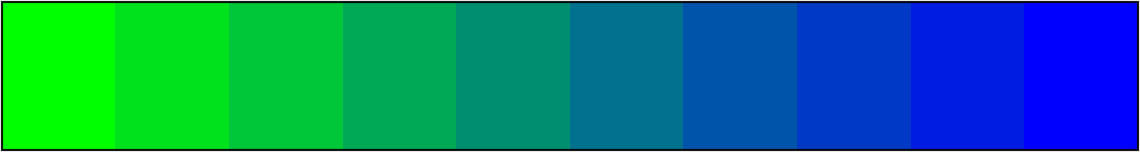
\includegraphics[width = 7cm]{\here/colorbarRGB.png}};
	\node[inner sep = 0pt, anchor = north, yshift = -0.2cm] (n2) at (n1.south)  {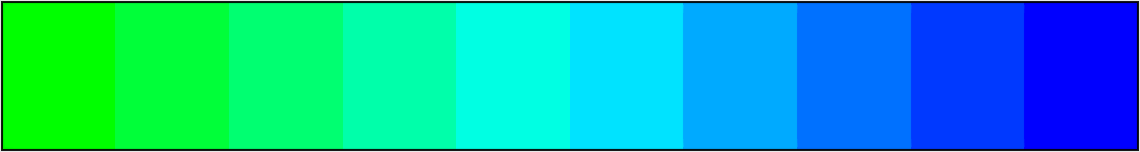
\includegraphics[width = 7cm]{\here/colorbarHSV.png}};
	\node[inner sep = 0pt, anchor = north, yshift = -0.2cm] (n3) at (n2.south) {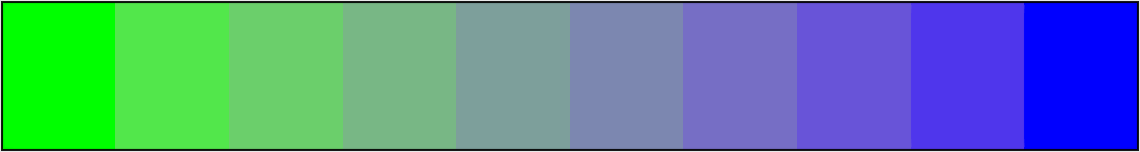
\includegraphics[width = 7cm]{\here/colorbarLab.png}};

	\node[anchor = east] at (n1.west){RGB};
	\node[anchor = east] at (n2.west){HSV};
	\node[anchor = east] at (n3.west){Lab};

\end{tikzpicture}
\end{minipage}
\end{figure} 


The key takeaway here is that a reasonable colors distance metric is not necessarily determined by an Eucledian color space distance, but by how the human eye and brain interpret those differences. A well-designed colormap is \emph{perceptually uniform}: Equal steps in the data should correspond to equal perceived changes in color---just as a fixed distance on the $x$ axis of a plot always represents the same step in scale. For example, in a topographic elevation map, a shift from 1500 meters to 1200 meters below sea level (represented by a change from dark to lighter blue) should be perceived as the same elevation increase as a shift from 1000 meters to 1300 meters above sea level (which might be represented by a transition from tan to a lighter tan).
Unsurprisingly, the human vision is a very complex issue and one that requires extensive empirical studies, see e.g. Refs.~\cite{rogowitz1996,mullen1985,crameri2020}. For example, research has shown that the human brain perceives changes in lightness far more effectively than changes in hue when interpreting data~\cite{rogowitz1996}. As a result, colormaps with a monotonically increasing lightness are generally more intuitive and easier to interpret for viewers.

\begin{figure}
	\centering
	\tikzsetnextfilename{fig_colordiffs}
	% tikz_colordiffs.tex

\begin{tikzpicture}

\begin{groupplot}[
		group style = {
			group name = dE,
			group size = 3 by 1,
			vertical sep = .25cm,
			horizontal sep = .25cm, 
			},
		width = 4.5cm,
		height = 4cm,
		enlargelimits = 0.05,
		simpleax1,
		ytick = {0,50,100},
		xticklabel = \empty,
		xmin = 0.5,
		xmax = 10.5,
		ymin = 0,
		ymax = 100,
		scale only axis,
		enlargelimits = false,
		xtick = {1.5,...,10.5},
		xmajorgrids = true, 
		ylabel = {lightness $L$},
		xlabel style = {yshift = -0.4cm},
		]

		\nextgroupplot[xlabel = {RGB}]
		\addplot+[hcqblue, ultra thick, mark = triangle*, mark options = {thin, fill = hcqblue, draw = black}]table[y index = 1]{coldiffLight.txt};
		%\coordinate (p1) at (rel axis cs:0,0);
		

		\nextgroupplot[xlabel = {HSV}, ylabel = \empty, yticklabel = \empty]
		\addplot+[hcqblue, ultra thick, mark = triangle*,mark options = {thin, fill = hcqblue, draw = black}]table[y index = 2]{coldiffLight.txt};

		\nextgroupplot[xlabel = {Lab}, ylabel = \empty, yticklabel = \empty]
		\addplot+[hcqblue, ultra thick, mark = triangle*,mark options = {thin, fill = hcqblue, draw = black}]table[y index = 3]{coldiffLight.txt};

\end{groupplot}

\node[draw = black, thick, inner sep = 0pt, anchor = north] at (dE c1r1.south){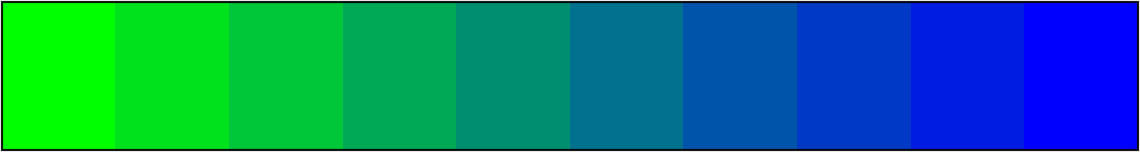
\includegraphics[width = 4.5cm]{\here/colorbarRGB.png}};
\node[draw = black, thick, inner sep = 0pt, anchor = north] at (dE c2r1.south){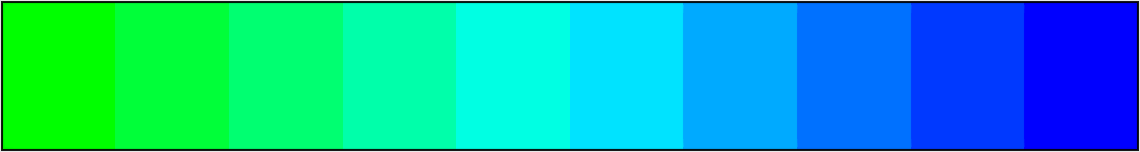
\includegraphics[width = 4.5cm]{\here/colorbarHSV.png}};
\node[draw = black, thick, inner sep = 0pt, anchor = north] at (dE c3r1.south){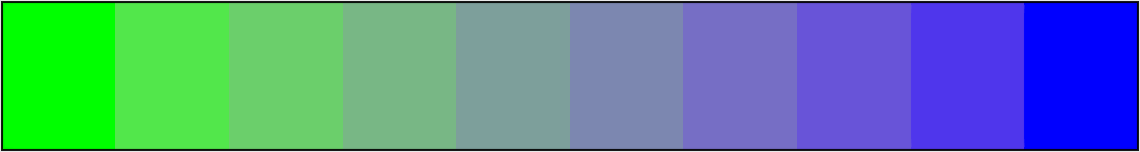
\includegraphics[width = 4.5cm]{\here/colorbarLab.png}};



\begin{groupplot}[
		group style = {
			group size = 3 by 1,
			vertical sep = .25cm,
			horizontal sep = .25cm, 
			},
		width = 4.5cm,
		height = 4cm,
		enlargelimits = 0.05,
		simpleax1,
		ytick = {0,12.5,25,37.5,50},
		xticklabel = \empty,
		yticklabels = {0,,,,50},
		xmin = 0.5,
		xmax = 10.5,
		ymin = 0,
		ymax = 50,
		ytick pos = right, 
		yticklabel pos = right,
		scale only axis,
		ylabel = {color difference},
		ylabel style = {yshift = 0.2cm},
		enlargelimits = false,
		xtick = {1.5,...,10.5},
		legend style = {
			at = {(0.5,1)},
			anchor = south,
			legend1},
		legend columns = 3
		]


		\nextgroupplot[ylabel = \empty, yticklabel = \empty]
		\addplot+[hcqyellow, ultra thick, mark options = {thin, fill = hcqyellow, draw = black}]table[y index = 1]{coldiffLab.txt};
		\addplot+[hcqred, ultra thick, mark options = {thin, fill = hcqred, draw = black}]table[y index = 1]{coldiff2000.txt};

		\addlegendentry{$\Delta E^*_{ab}$}
		\addlegendentry{$\Delta E^*_{2000}$}
		\addlegendimage{hcqblue, ultra thick, mark = triangle*, mark options = {thin, fill = hcqblue, draw = black}};
		\addlegendentry{$L$};
		

		\nextgroupplot[ylabel = \empty, yticklabel = \empty]
		\addplot+[hcqyellow, ultra thick, mark options = {thin, fill = hcqyellow, draw = black}]table[y index = 2]{coldiffLab.txt};
		\addplot+[hcqred, ultra thick, mark options = {thin, fill = hcqred, draw = black}]table[y index = 2]{coldiff2000.txt};

		\addlegendentry{$\Delta E^*_{ab}$}
		\addlegendentry{$\Delta E^*_{2000}$}
		\addlegendimage{hcqblue, ultra thick, mark = triangle*, mark options = {thin, fill = hcqblue, draw = black}};
		\addlegendentry{$L$};


		\nextgroupplot[]
		\addplot+[hcqyellow, ultra thick, mark options = {thin, fill = hcqyellow, draw = black}]table[y index = 3]{coldiffLab.txt};
		\addplot+[hcqred, ultra thick, mark options = {thin, fill = hcqred, draw = black}]table[y index = 3]{coldiff2000.txt};


		\addlegendentry{$\Delta E^*_{ab}$}
		\addlegendentry{$\Delta E^*_{2000}$}
		\addlegendimage{hcqblue, ultra thick, mark = triangle*, mark options = {thin, fill = hcqblue, draw = black}};
		\addlegendentry{$L$};

	\end{groupplot}

	\node[text width=1em, anchor=west]at(dE c1r1.north west){\subcaptionbox{\label{dEa}}{}};
	\node[text width=1em, anchor=west]at(dE c2r1.north west){\subcaptionbox{\label{dEb}}{}};
	\node[text width=1em, anchor=west]at(dE c3r1.north west){\subcaptionbox{\label{dEc}}{}};
\end{tikzpicture}

	\caption{\textbf{Lightness and color distances.} The three panels show the lightness $L$, as well as tow different color metrics for uniformely spaced in colors in (a) RGB, (b) HSV, and (c) Lab color space. For details, see the main text.}
	\label{fig:colordiffs}
\end{figure}

In \figref{fig:colordiffs}, we analyze the lightness (blue line) of the colors in the colormaps from \figref{fig:colorspaces} to see if our intuition (Lab is the best, followed by RGB, and then HSV) holds true.
The three panels confirm our anticipation:
\begin{itemize}
\item The RGB colors (left) exhibit a relatively constant change in lightness in the greenish range, but plateau near the blue end, making the last colors harder to distinguish.
\item The HSV colors (middle) maintain an almost constant lightness near the initial color, which matches our earlier judgment that the greenish hues are barely distinguishable.
\item The Lab colors (right) display a uniform decrease in lightness, ensuring well-distinguished colors throughout the entire range.
\end{itemize}

It is no coincidence that Lab performs best, as the Lab color space is designed to be perceptually uniform and maintain consistent perceptual differences when picking regularly spaced $(L,a,b)$ points. The $L$ component directly represents lightness. There are more color spaces designed to reflect human color vision, the earliest being CIEXYZ\footnote{CIE stands for Commission internationale de l'éclairage, which is french for International Commission on Illumination}, defined in 1931. It was developed using experimental data from human test subjects. However, CIEXYZ is not perceptually uniform, leading to the introduction of CIELAB (Lab) and CIELUV (Luv) in 1976, which aimed to address this limitation.

The CIE also introduced various color distance metrics, typically denoted as $\Delta E^*$, where $E$ stands for the German word `Empfindung'. The first definition, called $\Delta E^*_{ab}$, was simply the Eucledian distance in the Lab color space. As the understanding of human color perception evolved, non-uniformities in the CIELAB space, particularly in highly saturated regions, where discovered. To improve accuracy, better distance metrics were developed. The most advanced is CIEDE2000 $\Delta E^*_{00}$, which aligns with the latest research on human color vision. 
\figref{fig:colordiffs} also depicts $\Delta E^*_{ab}$ and $\Delta E^*_{00}$. 
Per definition, $\Delta E^*_{ab}$ remains constant for the Lab colors, while it peaks in the other two cases and decreases toward the edges. For $\Delta E^*_{00}$, the absolute magnitude is particularly significant: as noted earlier, colors in the green (HSV) and blue (RGB) regions are hard to distinguish. This is reflected in the $\Delta E^*_{00}$ values, which approach zero in those areas, whereas in the Lab space, a certain minimum distance is consistently maintained.


\subsection{Mach bands in diverging color maps}

Diverging colormaps typically pass through an unsaturated midpoint, often white. As a result, creating a perceptually uniform colormap by interpolating colors in the Lab color space (as done previously) is not possible. One possible approach is piecewise interpolation, i.e., moving from one color to white and then taking a sharp turn.  Such a sudden transition from increasing to decreasing lightness can activate the human eye's edge-detection mechanisms and create artificial visual features called Mach bands. It is often beneficial to soften the lightness gradient near the midpoint to avoid abrupt visual edges. This comes at the cost of a slight perceptual flat spot around the vanishing lightness gradient. For technical details on how to smoothen the lightness transition, see, e.g., Refs.~\cite{moreland2009,kovesi2015}.

\figref{fig:machbands} compares two diverging colormaps (taken from Ref.~\cite{moreland2009}) applied to the function $f(x) = \cos x + \cos y$. The colormaps share identical edge colors, but (a) has a sharp peak in lightness, while (c) has a smoother transition. The respective lightness values are shown in panel (b). In (a), the peak creates white Mach bands, whereas in (c), these artificial features are absent, thanks to the flattened lightness transition.
While (c) may be preferable in many situations, it is not always the better choice. In some cases, a sharp transition can be desirable, especially when the white midpoint carries specific significance. For example, in \figref{fig:machbands}, the contour lines where $f(x)=0$ could represent the Fermi lines of a square lattice tight-binding model. If the goal is to highlight the precise shape of the Fermi line, a sharp contrast can be advantageous.

In summary, when selecting a diverging colormap, be mindful of potential artifacts and carefully consider whether these are undesirable or beneficial.

\begin{figure}
	\centering
	\tikzsetnextfilename{fig_machbands}
	% This is the Mach band plot.
\begin{tikzpicture} 
	\begin{groupplot}[
		group style = {
			group name = name1,
			group size = 3 by 1,
			vertical sep = .25cm,
			horizontal sep = .15cm, 
			},
			view={0}{90},
			simpleax1,
			width = .7*\axisdefaultwidth,
			height = .7*\axisdefaultwidth,
			simpleax1,
			xtick = {-6.28,0,6.28},
			xticklabels = {$-2\pi$, $0$, $2\pi$},
			ytick = {-6.28,0,6.28},
			yticklabels = {$-2\pi$, $0$, $2\pi$},
			xlabel = $x$,
			ylabel = $y$,
			scatter/use mapped color={
       			draw=black,
        		fill=mapped color,
    		}, 
			ylabel style = {yshift = -0.4cm},
			colorbar horizontal,
			colorbar style={
					axis line style = {line cap=rect},
					ticklabel style = {font=\footnotesize},
					thick,
					at={(0,1.02)},            
					anchor=below south west, 
					width=1*\pgfkeysvalueof{/pgfplots/parent axis width},
					xticklabel pos=upper,
					xlabel = {$f(x)$},
					axis on top,
					xtick pos=right,
					xlabel near ticks
				}, 
		]
	
		\nextgroupplot[colormap name = coolwarmB, colorbar] 
		\addplot3[surfstyle, domain=-6.29:6.29]{cos(deg(y)) + cos(deg(x))}; 

		\nextgroupplot[xmin=0, xmax=100, xshift = .6cm, ylabel = {lightness $L$}, xlabel = color, xtick = \empty, ymin = 37, ymax = 100, ytick = {40, 100}, yticklabels = {40, 100}, colorbar = false, ylabel style = {yshift = -0.3cm},]
		\addplot[colormap name = coolwarm, scatter, scatter src = x, ultra thin] table[]{machbands2.txt};
		\addplot[colormap name = coolwarmB, scatter, scatter src = x, ultra thin] table[y index = 2]{machbands2.txt};
		\coordinate (m1) at (axis cs: 50.0, 94.662);
		\coordinate (m2) at (axis cs: 75.0, 72.33121);

		\nextgroupplot[colormap name = coolwarm, ytick pos = right, yticklabel pos = right, ylabel style = {yshift = 0.8cm}]
		\addplot3[surfstyle, domain=-6.29:6.29]{cos(deg(y)) + cos(deg(x))}; 

	\end{groupplot} 

	\draw[-stealth, ultra thick, hcqblue] (m1) -- (m1 -| name1 c1r1.east);
	\draw[-stealth, ultra thick, hcqblue] (m2) -- (m2 -| name1 c3r1.west);

	\node[yshift = 0.3cm, text width = 1em, anchor = south east]at (name1 c1r1.north west) {\subcaptionbox{\label{mach-a}}{}};
	\node[yshift = 0.3cm, text width = 1em, anchor = south east]at (name1 c2r1.north west) {\subcaptionbox{\label{mach-b}}{}};
	\node[yshift = 0.3cm, text width = 1em, anchor = south east]at (name1 c3r1.north west) {\subcaptionbox{\label{mach-c}}{}};


\end{tikzpicture}

	\caption{\textbf{Mach bands in diverging colormaps.} Shown is the function $f(x) = \cos x + \cos y$, color-coded with a colormap with (a) a sharp change in lightness at the white point, resulting in white Mach bands and (c) a smoothened lightness evolution. Panel (b) shows the lightness values $L$ for the two colormaps.}
	\label{fig:machbands}
\end{figure}


\section{An example: Rainbow vs. good colormaps}\label{sec:rainbow}

To end this section, let us look at an exampler that illustrates the advantages of a good scientifically derived colormap and some serious drawbacks of a bad colormap. We will look at a two-dimensional plot of the function $f(x)= \ldots$



\subsection{The original colormap}
\subsection{Color vision deficiency}


% \begin{figure}
% 	\centering
% 	\tikzsetnextfilename{fig_colorbars}
% 	% tikz_colorbars.tex

\begin{tikzpicture} 
	
	\node[inner sep = 0pt] (c1) {
\includegraphics[width = 4.1cm]{\here/colorbars/cividis.png}};
	\node[inner sep = 0pt, anchor = north, yshift = -0.1cm] (c2) at (c1.south)  {
\includegraphics[width = 4.1cm]{\here/colorbars/cividis_prot.png}};
	\node[inner sep = 0pt, anchor = north, yshift = -0.1cm] (c3) at (c2.south) {
\includegraphics[width = 4.1cm]{\here/colorbars/cividis_deut.png}};
	\node[inner sep = 0pt, anchor = north, yshift = -0.1cm] (c4) at (c3.south) {
\includegraphics[width = 4.1cm]{\here/colorbars/cividis_trit.png}};
	\node[inner sep = 0pt, anchor = north, yshift = -0.1cm] (c5) at (c4.south) {
\includegraphics[width = 4.1cm]{\here/colorbars/cividis_mono.png}};


	\node[anchor = west, xshift = 0.1cm, inner sep = 0pt] (b1) at (c1.east) {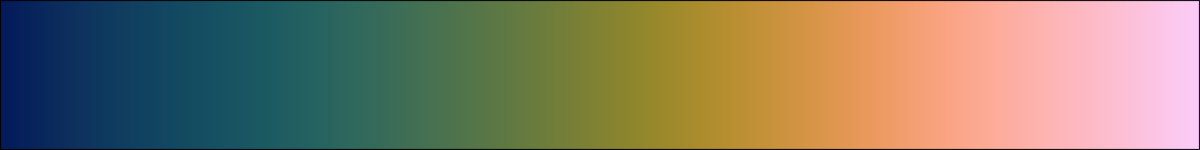
\includegraphics[width = 4.1cm]{\here/colorbars/batlow.png}};
	\node[inner sep = 0pt, anchor = north, yshift = -0.1cm] (b2) at (b1.south)  {
\includegraphics[width = 4.1cm]{\here/colorbars/batlow_prot.png}};
	\node[inner sep = 0pt, anchor = north, yshift = -0.1cm] (b3) at (b2.south) {
\includegraphics[width = 4.1cm]{\here/colorbars/batlow_deut.png}};
	\node[inner sep = 0pt, anchor = north, yshift = -0.1cm] (b4) at (b3.south) {
\includegraphics[width = 4.1cm]{\here/colorbars/batlow_trit.png}};
	\node[inner sep = 0pt, anchor = north, yshift = -0.1cm] (b5) at (b4.south) {
\includegraphics[width = 4.1cm]{\here/colorbars/batlow_mono.png}};


	\node[anchor = west, xshift = 0.1cm, inner sep = 0pt] (r1) at (b1.east) {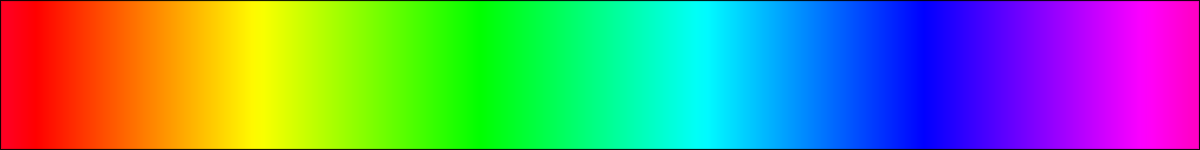
\includegraphics[width = 4.1cm]{\here/colorbars/rb.png}};
	\node[inner sep = 0pt, anchor = north, yshift = -0.1cm] (r2) at (r1.south)  {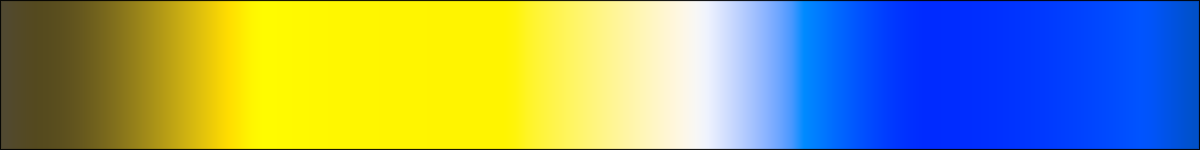
\includegraphics[width = 4.1cm]{\here/colorbars/rb_prot.png}};
	\node[inner sep = 0pt, anchor = north, yshift = -0.1cm] (r3) at (r2.south) {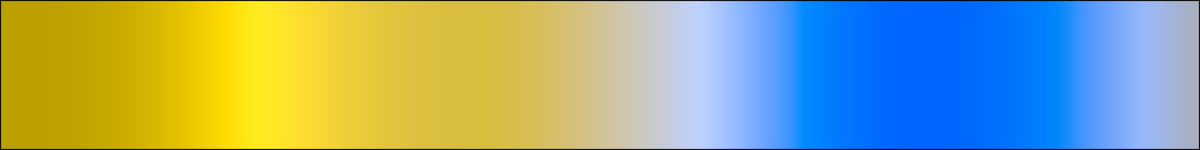
\includegraphics[width = 4.1cm]{\here/colorbars/rb_deut.png}};
	\node[inner sep = 0pt, anchor = north, yshift = -0.1cm] (r4) at (r3.south) {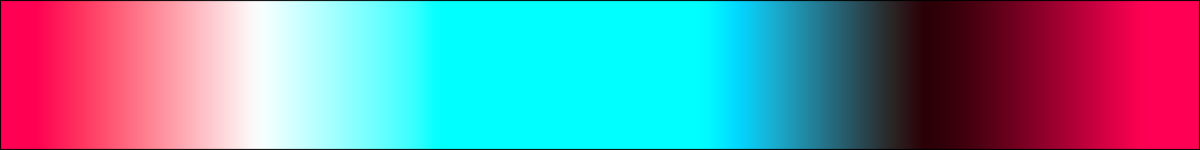
\includegraphics[width = 4.1cm]{\here/colorbars/rb_trit.png}};
	\node[inner sep = 0pt, anchor = north, yshift = -0.1cm] (r5) at (r4.south) {
\includegraphics[width = 4.1cm]{\here/colorbars/rb_mono.png}};

	\node[anchor = east, font = \footnotesize] at (c1.west){original};
	\node[anchor = east, font = \footnotesize] at (c2.west){protanopia};
	\node[anchor = east, font = \footnotesize] at (c3.west){deuteranopia};
	\node[anchor = east, font = \footnotesize] at (c4.west){tritanopia};
	\node[anchor = east, font = \footnotesize] at (c5.west){monochrome};

	\node[anchor = south, font = \footnotesize] at (c1.north){\texttt{cividis}};
	\node[anchor = south, font = \footnotesize] at (b1.north){\texttt{batlow}};
	\node[anchor = south, font = \footnotesize] at (r1.north){\texttt{gist\_rainbow}};

\end{tikzpicture}
% 	\caption{xxx}
% 	\label{fig:colorbars}
% \end{figure}


% \begin{figure}
% 	\centering
% 	\tikzsetnextfilename{fig_sensitivityfunction}
% 	% tikz_sensitivityfunction.tex


\begin{tikzpicture}
	\begin{axis}[
			view={0}{90},
			simpleax1,
			xtick = {1,2,3},
			ytick = {0,0.5,1},
			xlabel = $x$,
			ylabel = $y$,
			colorbar horizontal,
			colorbar style={
					axis line style = {line cap=rect},
					ticklabel style = {font=\footnotesize},
					thick,
					at={(0,1.02)},   
					% xtick = {-1.5,0,1.5},       
					anchor=below south west, 
					width=1*\pgfkeysvalueof{/pgfplots/parent axis width},
					xticklabel pos=upper,
					xlabel = {$f(x)$},
					axis on top,
					xtick pos=right,
					xlabel near ticks,
				}, 
			colormap name = viridis
		]
	
		\addplot3[samples = 100, surfstyle, domain=0.7:3, y domain = 0:1]{(1 - y ^(1/2)) * cos(deg(x^3))}; 
	
	\end{axis}
\end{tikzpicture}
% 	\caption{xxx}
% 	\label{fig:sensitivityfunction}
% \end{figure}


% \begin{figure}
% 	\centering
% 	\tikzsetnextfilename{fig_sensitivityCVD}
% 	% tikz_sensitivityCVD.tex

\begin{tikzpicture} 
	
	\node[draw = black, thick, inner sep = 0pt] (c11) {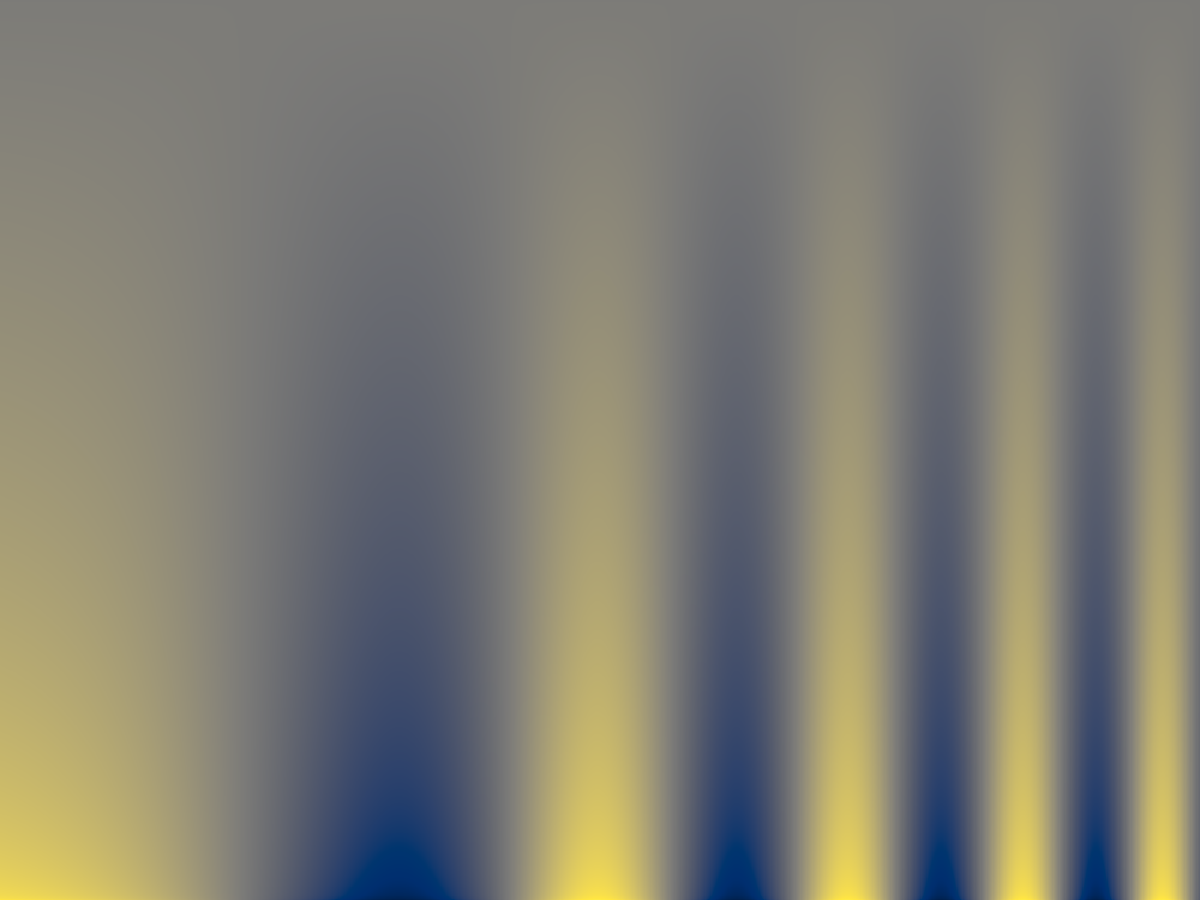
\includegraphics[width = 4.5cm]{\here/sensitivity/sensitivity_11.png}};
	\node[draw = black, thick, inner sep = 0pt, anchor = north, yshift = -0.2cm] (c21) at (c11.south)  {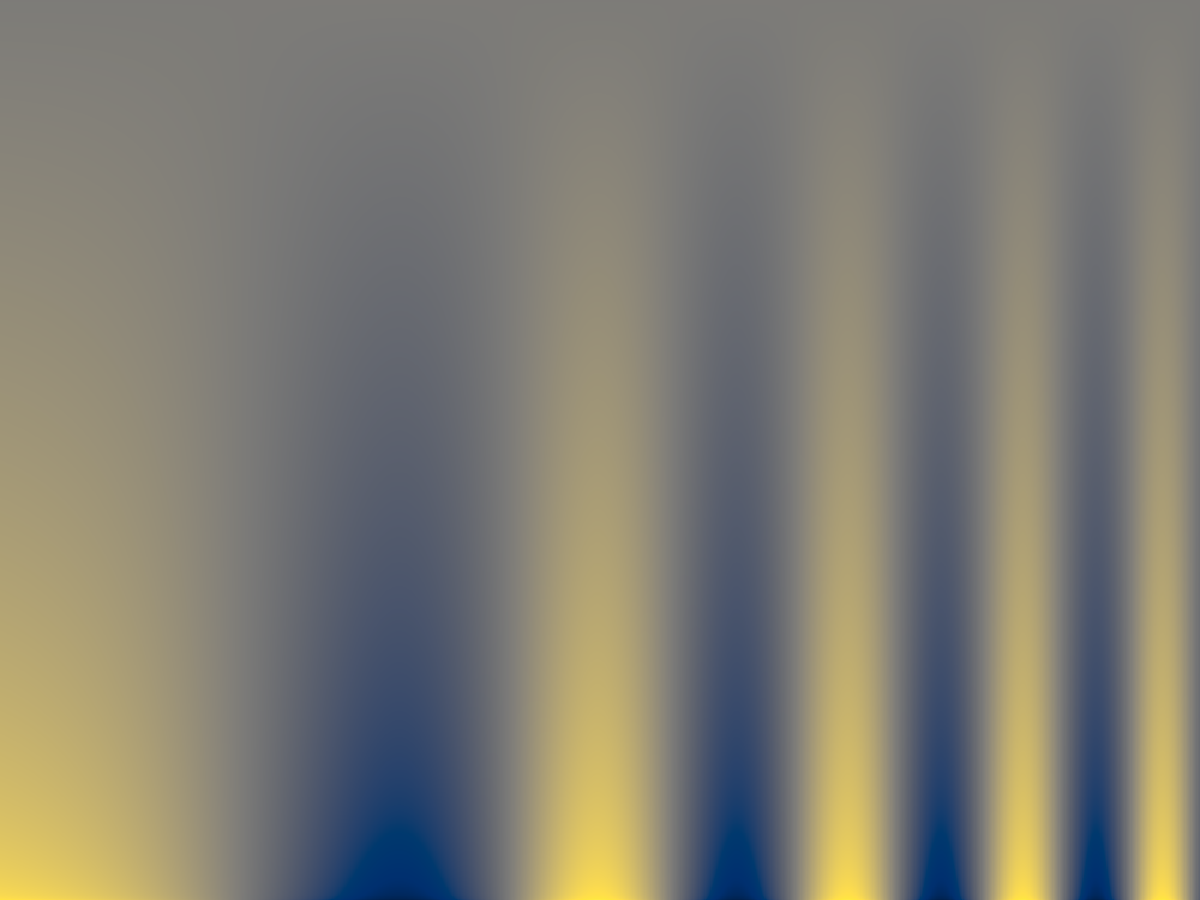
\includegraphics[width = 4.5cm]{\here/sensitivity/sensitivity_21.png}};
	\node[draw = black, thick, inner sep = 0pt, anchor = north, yshift = -0.2cm] (c31) at (c21.south) {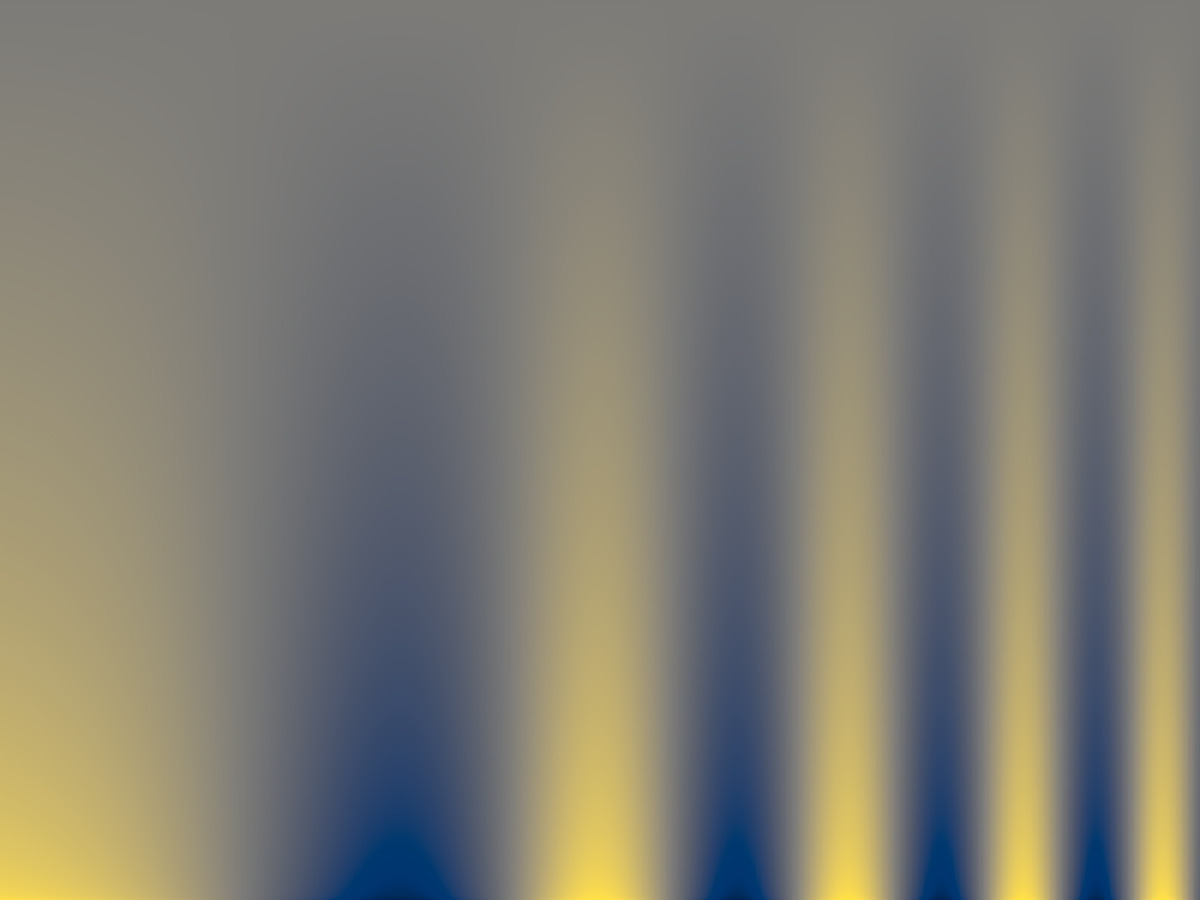
\includegraphics[width = 4.5cm]{\here/sensitivity/sensitivity_31.png}};
	\node[draw = black, thick, inner sep = 0pt, anchor = north, yshift = -0.2cm] (c41) at (c31.south) {
\includegraphics[width = 4.5cm]{\here/sensitivity/sensitivity_41.png}};
	\node[draw = black, thick, inner sep = 0pt, anchor = north, yshift = -0.2cm] (c51) at (c41.south) {
\includegraphics[width = 4.5cm]{\here/sensitivity/sensitivity_51.png}};

	\node[draw = black, thick, inner sep = 0pt, anchor = west, xshift = 0.3cm] (b12) at (c11.east){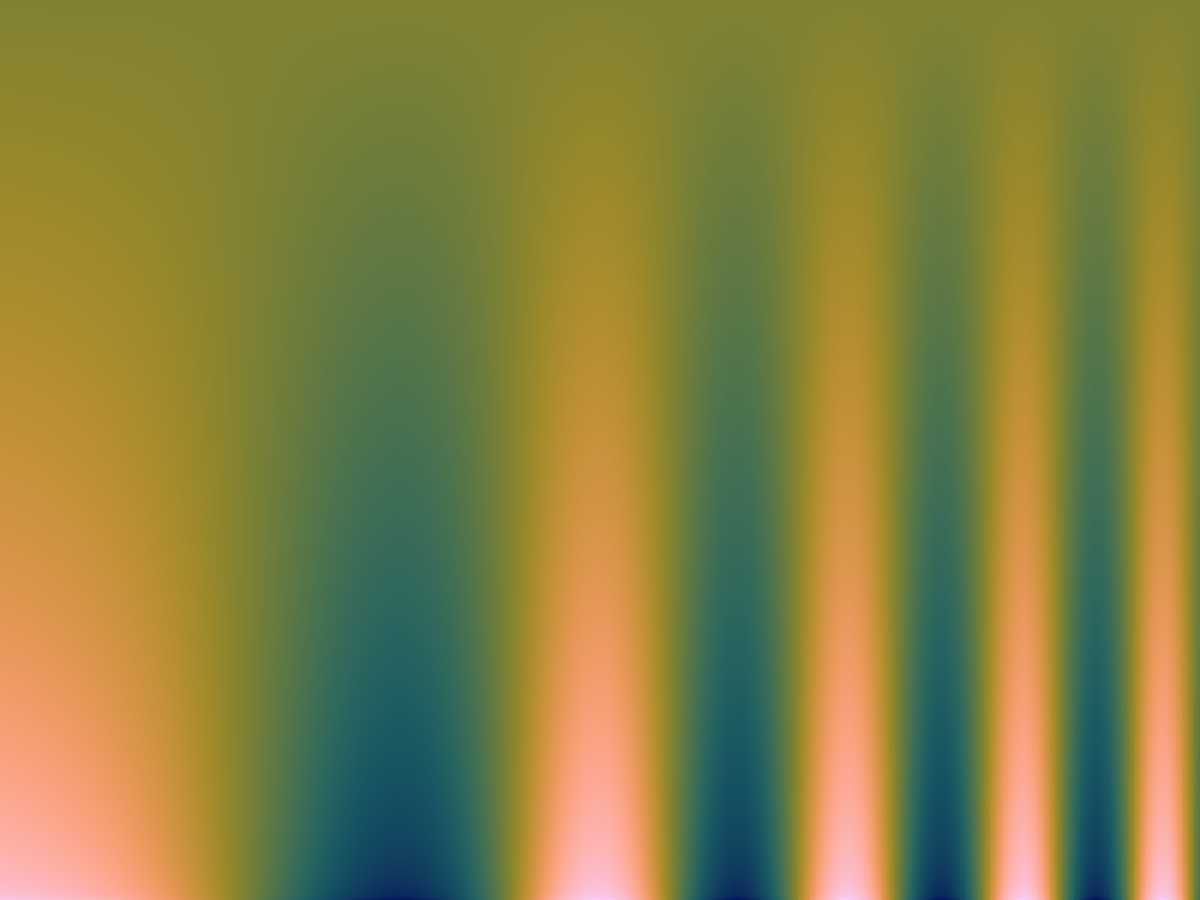
\includegraphics[width = 4.5cm]{\here/sensitivity/sensitivity_12.png}};
	\node[draw = black, thick, inner sep = 0pt, anchor = north, yshift = -0.2cm] (b22) at (b12.south)  {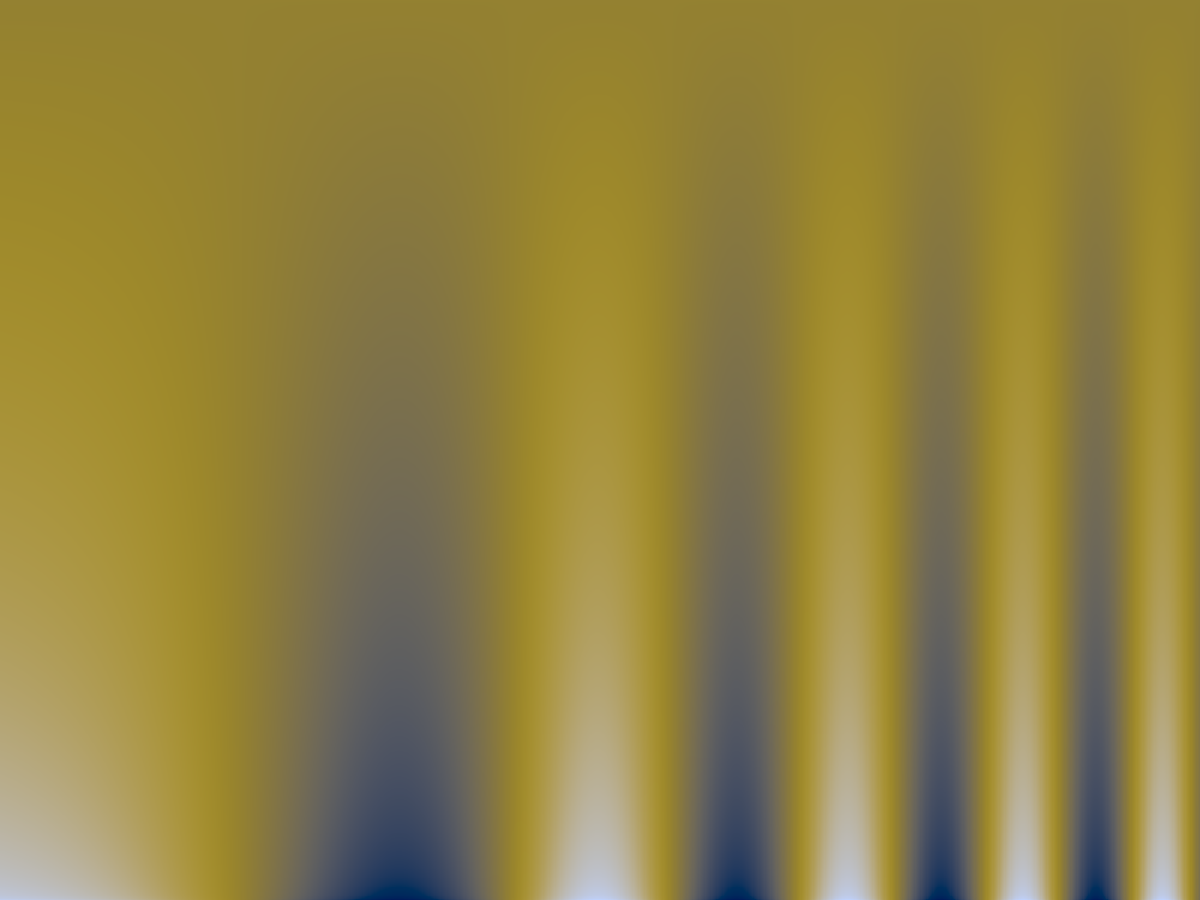
\includegraphics[width = 4.5cm]{\here/sensitivity/sensitivity_22.png}};
	\node[draw = black, thick, inner sep = 0pt, anchor = north, yshift = -0.2cm] (b32) at (b22.south) {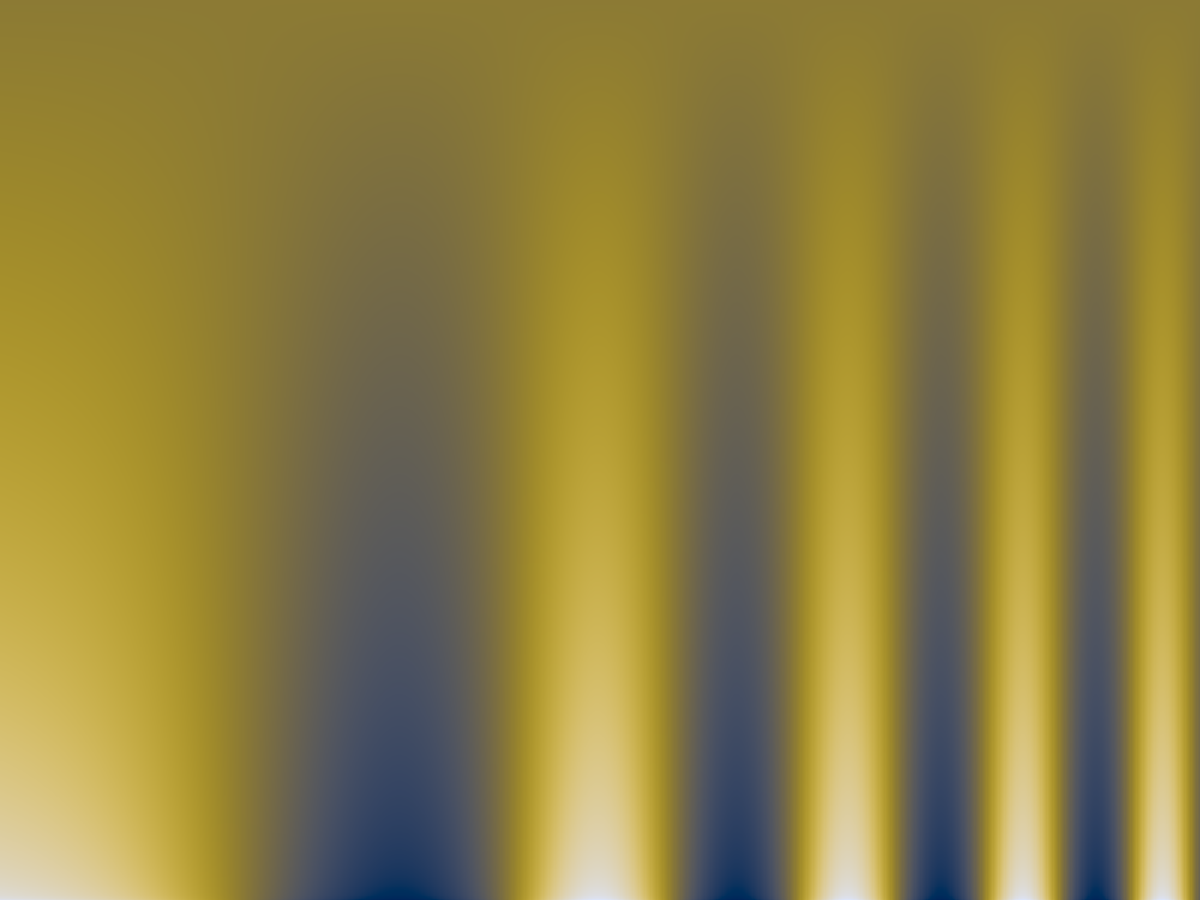
\includegraphics[width = 4.5cm]{\here/sensitivity/sensitivity_32.png}};
	\node[draw = black, thick, inner sep = 0pt, anchor = north, yshift = -0.2cm] (b42) at (b32.south) {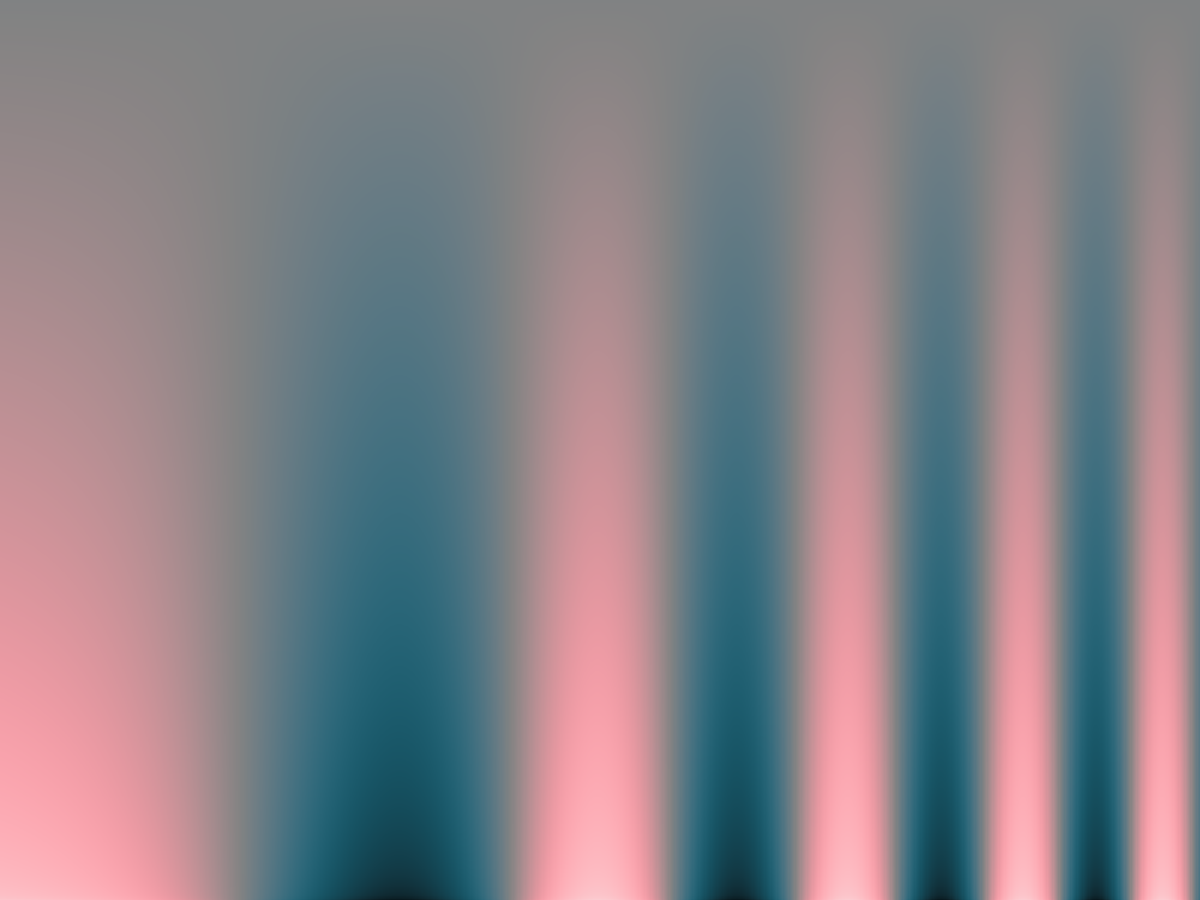
\includegraphics[width = 4.5cm]{\here/sensitivity/sensitivity_42.png}};
	\node[draw = black, thick, inner sep = 0pt, anchor = north, yshift = -0.2cm] (b52) at (b42.south) {
\includegraphics[width = 4.5cm]{\here/sensitivity/sensitivity_52.png}};


	\node[draw = black, thick, inner sep = 0pt, anchor = west, xshift = 0.3cm] (r12) at (b12.east){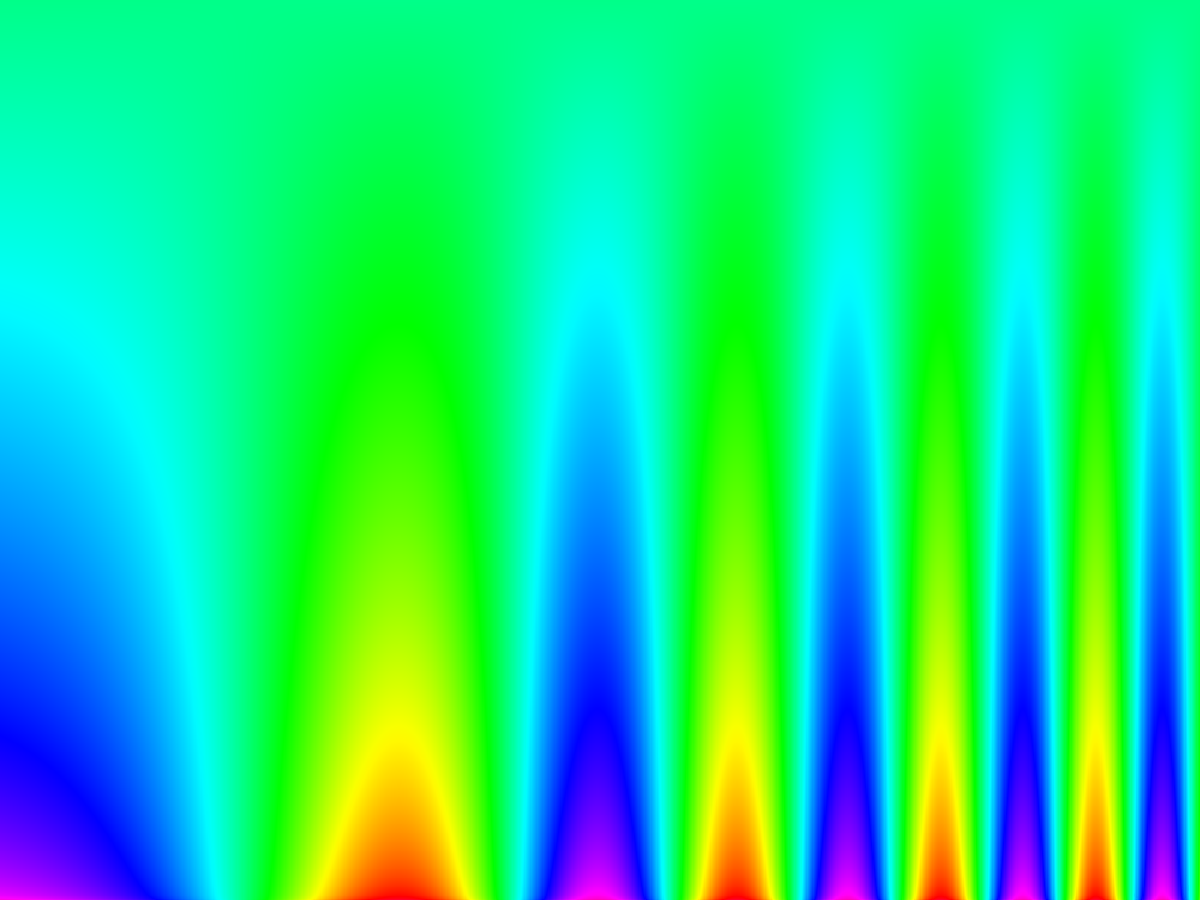
\includegraphics[width = 4.5cm]{\here/sensitivity/sensitivity_13.png}};
	\node[draw = black, thick, inner sep = 0pt, anchor = north, yshift = -0.2cm] (r22) at (r12.south)  {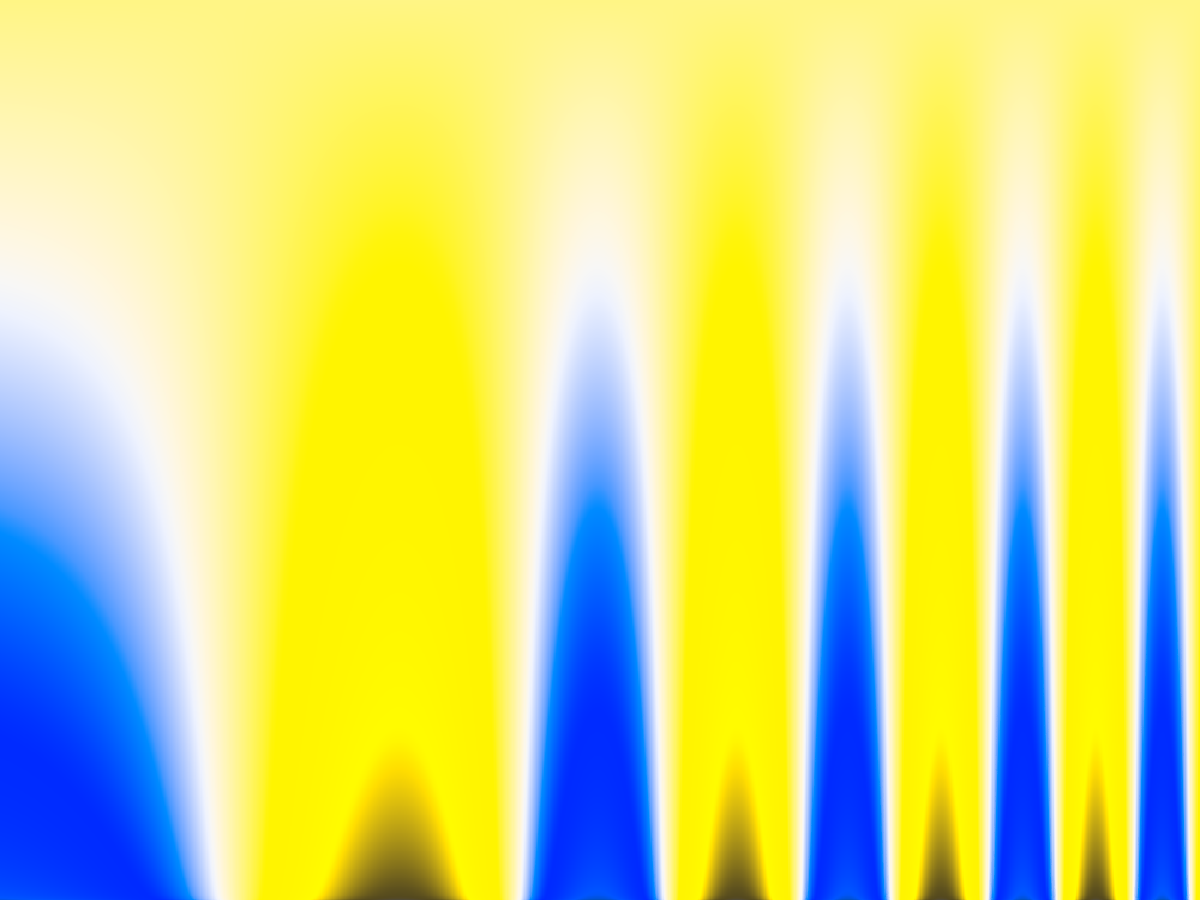
\includegraphics[width = 4.5cm]{\here/sensitivity/sensitivity_23.png}};
	\node[draw = black, thick, inner sep = 0pt, anchor = north, yshift = -0.2cm] (r32) at (r22.south) {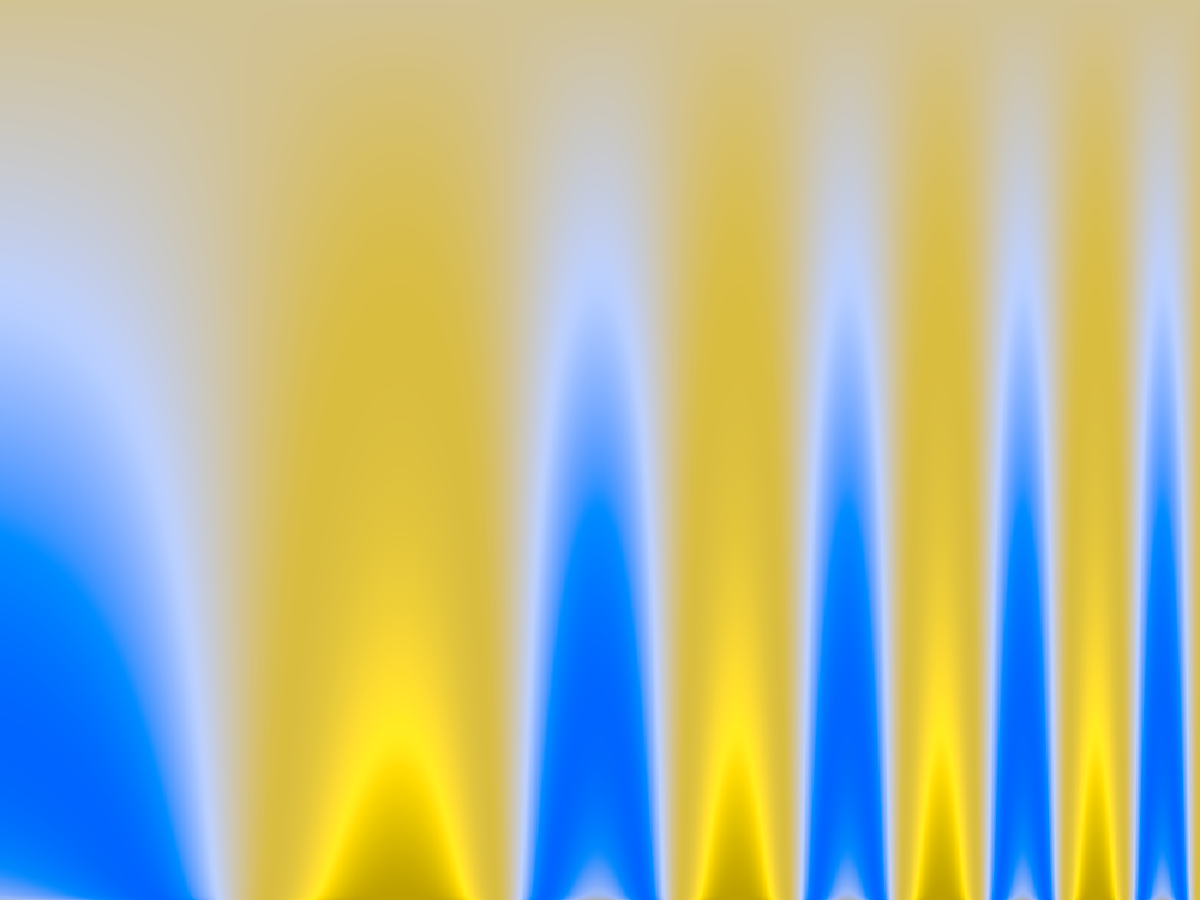
\includegraphics[width = 4.5cm]{\here/sensitivity/sensitivity_33.png}};
	\node[draw = black, thick, inner sep = 0pt, anchor = north, yshift = -0.2cm] (r42) at (r32.south) {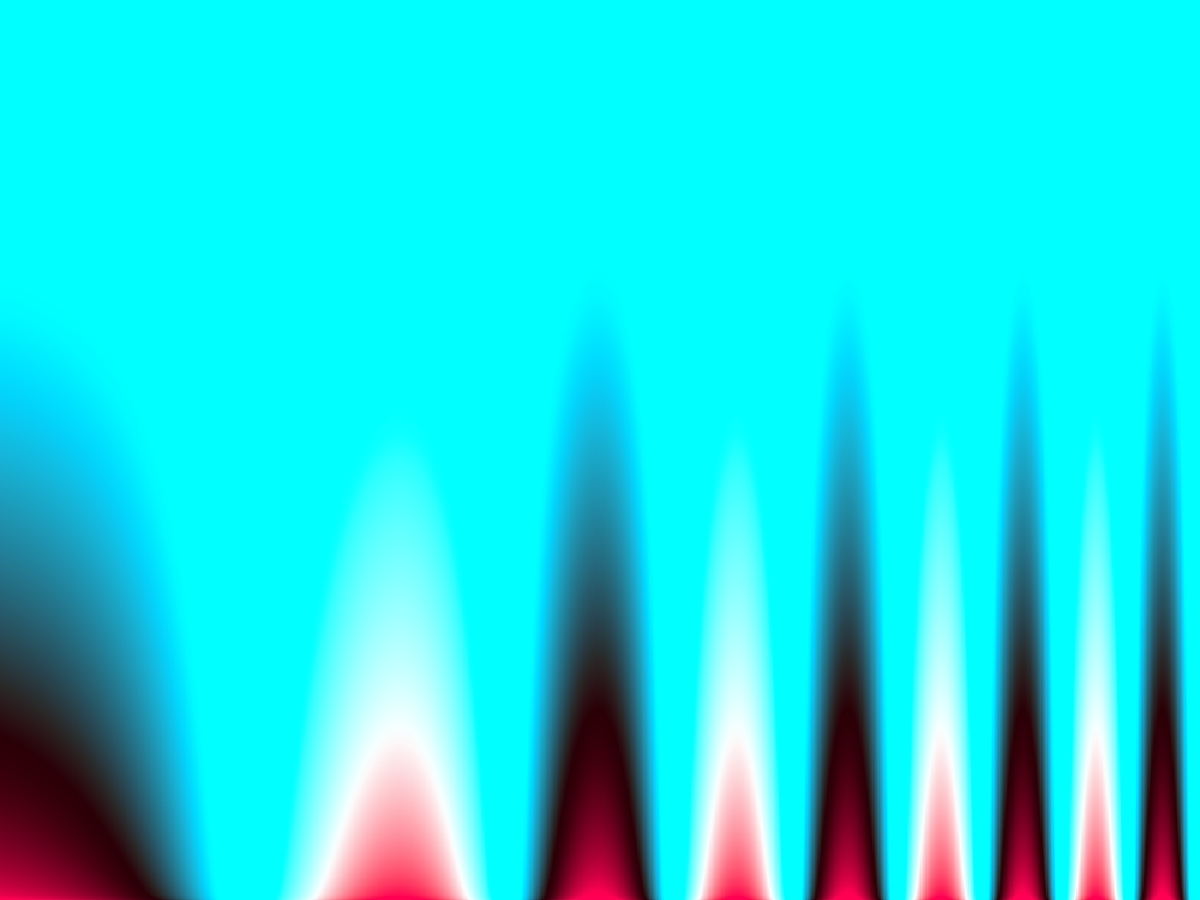
\includegraphics[width = 4.5cm]{\here/sensitivity/sensitivity_43.png}};
	\node[draw = black, thick, inner sep = 0pt, anchor = north, yshift = -0.2cm] (r52) at (r42.south) {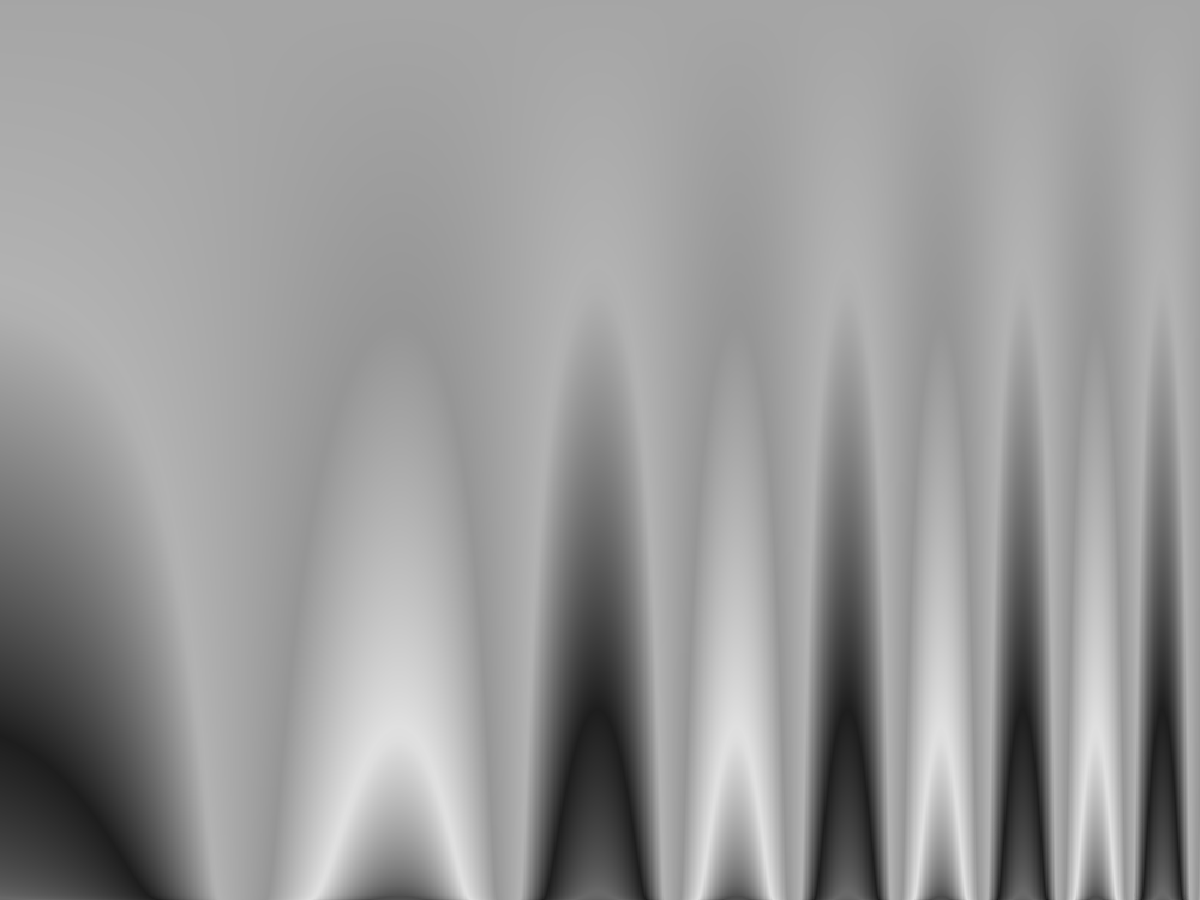
\includegraphics[width = 4.5cm]{\here/sensitivity/sensitivity_53.png}};


	\node[font = \footnotesize, anchor = east] at (c11.west){\rotatebox{90}{original}};
	\node[font = \footnotesize, anchor = east] at (c21.west){\rotatebox{90}{protanopia}};
	\node[font = \footnotesize, anchor = east] at (c31.west){\rotatebox{90}{deuteranopia}};
	\node[font = \footnotesize, anchor = east] at (c41.west){\rotatebox{90}{tritanopia}};
	\node[font = \footnotesize, anchor = east] at (c51.west){\rotatebox{90}{monochrome}};

	\node[anchor = south] at (c11.north){\texttt{cividis}};
	\node[anchor = south] at (b12.north){\texttt{batlow}};
	\node[anchor = south] at (r12.north){\texttt{gist\_rainbow}};

\end{tikzpicture}
% 	\caption{xxx}
% 	\label{fig:sensitivityCVD}
% \end{figure}

% \begin{figure}
% 	\centering
% 	\tikzsetnextfilename{fig_cmapanalytics}
% 	% tikz_cmapanalytics.tex
\pgfplotsset{
	simpleax1/.style = {
		every x tick/.style={black},
		every y tick/.style={black},
		xtick pos=left,
		ytick pos=left,
		axis on top,
		axis line style={thick, line cap = rect},
		ticklabel style = {font=\footnotesize}
	},
	surfstyle/.style = {
		surf, 
		shader=interp,
        samples=100,
	},
	colormap/RdBu,
	legend1/.style = 
	{
		font = \footnotesize,
		legend cell align={left},
		draw = none,
		/pgfplots/legend image code/.code={
			\draw[mark repeat=2,mark phase=2] 
			plot coordinates {
				(0cm,0cm) 
				(0.2cm,0cm)
				(0.4cm,0cm)
			};
		}
	},
}


\begin{tikzpicture}

\begin{groupplot}[
		group style = {
			group name = group1,
			group size = 3 by 1,
			vertical sep = .25cm,
			horizontal sep = .1cm, 
			},
		width = 4.25cm,
		height = 4cm,
		enlargelimits = 0.05,
		simpleax1,
		xticklabel = \empty,
		ymin = 0,
		ymax = 5.5,
		scatter/use mapped color={
       		draw=black,
        	fill=mapped color,
    	}, 
		scale only axis,
		enlargelimits = false, 
		ylabel = {$L$},
		ylabel style = {yshift = -0.5cm},
		legend style = {
			at = {(0.5,1)},
			anchor = south,
			legend1},
		legend columns = 3
		]

		\nextgroupplot[ytick = {0,100}, ymax = 100, ylabel = {lightness $L$}]
		\addplot[hcqblue, ultra thick]table[]{cmap_analytics/cv_L.txt};
		% \addplot[colormap/viridis, scatter, scatter src = x, ultra thin]table[]{cmap_analytics/cv_L.txt};
		\addplot[hcqyellow, ultra thick]table[]{cmap_analytics/bt_L.txt};



		\nextgroupplot[ylabel style = {yshift = 0.4cm}, ylabel = $\Delta E^*_{00}$, xshift = .9cm]
		\addplot[hcqblue, ultra thick]table[y expr =  4 *\thisrowno{1}]{cmap_analytics/cv_d.txt};
		\addplot[hcqyellow, ultra thick]table[y expr =  4*\thisrowno{1}]{cmap_analytics/bt_d.txt};

		\addlegendentry{\texttt{cividis}}
		\addlegendentry{\texttt{batlow}}
		\addlegendimage{hcqred, ultra thick};
		\addlegendentry{\texttt{gist\_rainbow}};


		\nextgroupplot[ymax = 100, ylabel = {$\Delta E_{00}^{\text{cum}}$}, ytick pos = right, yticklabel pos = right, ytick = {0,100}, ylabel style = {yshift = 0.8cm}]
		\addplot[hcqblue, ultra thick]table[]{cmap_analytics/cv_d_cum.txt};
		\addplot[hcqyellow, ultra thick]table[]{cmap_analytics/bt_d_cum.txt};


\end{groupplot}

\node[draw = black, thick, inner sep = 0pt, anchor = north] (cb1) at (group1 c1r1.south){
\includegraphics[width = 4.25cm, height = .3cm]{\here/colorbars/cividis.png}};
\node[draw = black, thick, inner sep = 0pt, anchor = north] (cb2) at (cb1.south){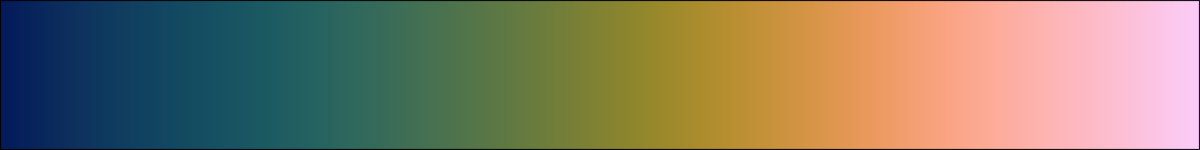
\includegraphics[width = 4.25cm, height = .3cm]{\here/colorbars/batlow.png}};
\node[draw = black, thick, inner sep = 0pt, anchor = north] (cb3) at (cb2.south){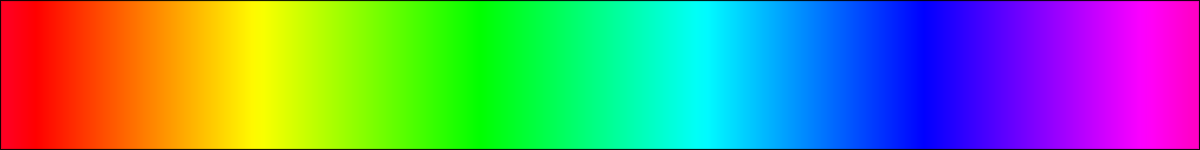
\includegraphics[width = 4.25cm, height = .3cm]{\here/colorbars/rb.png}};


\node[draw = black, thick, inner sep = 0pt, anchor = north] (cb4) at (group1 c2r1.south){
\includegraphics[width = 4.25cm, height = .3cm]{\here/colorbars/cividis.png}};
\node[draw = black, thick, inner sep = 0pt, anchor = north] (cb5) at (cb4.south){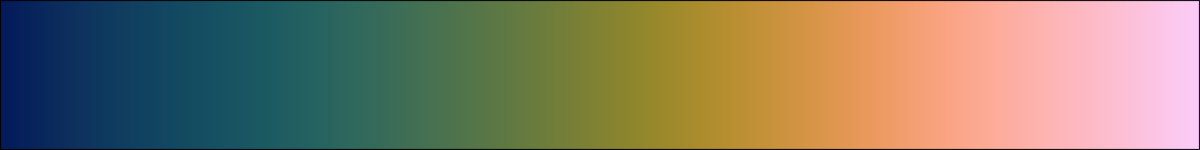
\includegraphics[width = 4.25cm, height = .3cm]{\here/colorbars/batlow.png}};
\node[draw = black, thick, inner sep = 0pt, anchor = north] (cb6) at (cb5.south){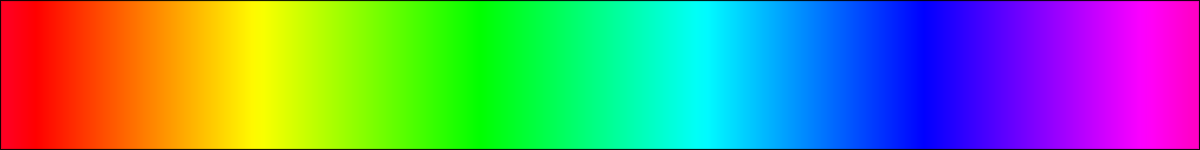
\includegraphics[width = 4.25cm, height = .3cm]{\here/colorbars/rb.png}};


\node[draw = black, thick, inner sep = 0pt, anchor = north] (cb7) at (group1 c3r1.south){
\includegraphics[width = 4.25cm, height = .3cm]{\here/colorbars/cividis.png}};
\node[draw = black, thick, inner sep = 0pt, anchor = north] (cb8) at (cb7.south){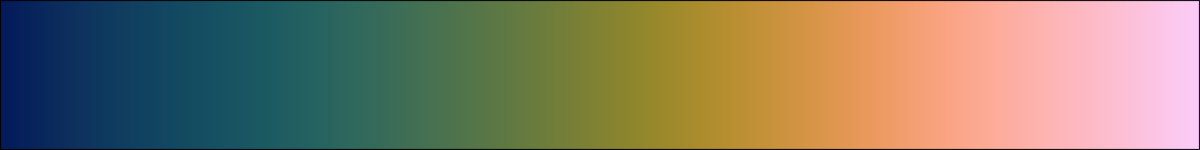
\includegraphics[width = 4.25cm, height = .3cm]{\here/colorbars/batlow.png}};
\node[draw = black, thick, inner sep = 0pt, anchor = north] (cb9) at (cb8.south){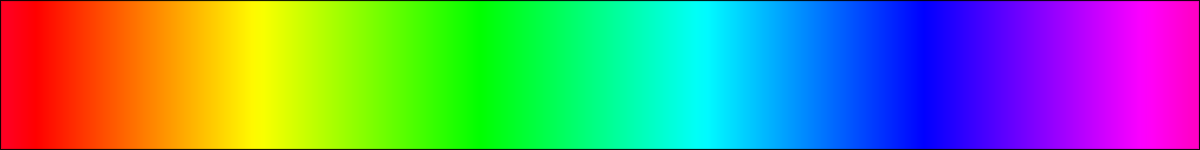
\includegraphics[width = 4.25cm, height = .3cm]{\here/colorbars/rb.png}};

\begin{groupplot}[
		group style = {
			group size = 3 by 1,
			vertical sep = .25cm,
			horizontal sep = .1cm, 
			},
		width = 4.25cm,
		height = 4cm,
		enlargelimits = 0.05,
		simpleax1,
		% ytick = {0,50},
		xticklabel = \empty,
		% xmin = 0.5,
		% xmax = 10.5,
		ymin = 0,
		ymax = 5.5,
		ytick pos = right, 
		yticklabel pos = right,
		scale only axis,
		enlargelimits = false,
		% xtick = {1.5,...,10.5},
		legend style = {
			at = {(0.5,1)},
			anchor = south,
			legend1},
		legend columns = 3,
		xtick = \empty,
		]


		\nextgroupplot[ymax = 100, ylabel = \empty, yticklabel = \empty]
		\addplot[ultra thick, hcqred]table[]{cmap_analytics/rb_L.txt};

		\nextgroupplot[xshift = .9cm, ylabel = \empty, yticklabel = \empty]
		\addplot[ultra thick, hcqred]table[y index = 1]{cmap_analytics/rb_d.txt};
		
		% \addlegendentry{$\Delta E^*_{ab}$}
		% \addlegendentry{$\Delta E^*_{2000}$}
		% \addlegendimage{hcqblue, ultra thick, mark = triangle*, mark options = {thin, fill = hcqblue, draw = black}};
		% \addlegendentry{$L$};
		

		\nextgroupplot[ylabel = \empty, yticklabel = \empty, ymax = 100, ytick pos = right, yticklabel pos = right]
		\addplot[hcqred, ultra thick]table[]{cmap_analytics/rb_d_cum.txt};
		% \addplot+[hcqred, ultra thick, mark options = {thin, fill = hcqred, draw = black}]table[y index = 2]{coldiff2000.txt};

		% \addlegendentry{$\Delta E^*_{ab}$}
		% \addlegendentry{$\Delta E^*_{2000}$}
		% \addlegendimage{hcqblue, ultra thick, mark = triangle*, mark options = {thin, fill = hcqblue, draw = black}};
		% \addlegendentry{$L$};


		% \nextgroupplot[]
		% \addplot+[hcqyellow, ultra thick, mark options = {thin, fill = hcqyellow, draw = black}]table[y index = 3]{coldiffLab.txt};
		% \addplot+[hcqred, ultra thick, mark options = {thin, fill = hcqred, draw = black}]table[y index = 3]{coldiff2000.txt};


		% \addlegendentry{$\Delta E^*_{ab}$}
		% \addlegendentry{$\Delta E^*_{2000}$}
		% \addlegendimage{hcqblue, ultra thick, mark = triangle*, mark options = {thin, fill = hcqblue, draw = black}};
		% \addlegendentry{$L$};

	\end{groupplot}

	\node[text width=1em, anchor=west]at(group1 c1r1.north west){\subcaptionbox{\label{cmA}}{}};
	\node[text width=1em, anchor=west]at(group1 c2r1.north west){\subcaptionbox{\label{cmB}}{}};
	\node[text width=1em, anchor=west]at(group1 c3r1.north west){\subcaptionbox{\label{cmC}}{}};
\end{tikzpicture}

% 	\caption{Note: Scales are not directly comparable! But shape of each individual line is what matters here.}
% 	\label{fig:cmapanalytics}
% \end{figure}



% Here is how you define a new ColorScheme:
% \begin{listing}[h]
% \begin{minted}[xleftmargin = 1.5cm]{julia} 
% using Colors, ColorSchemes
% cividis_cols = ColorSchemes.cividis.colors
% cividis_protanopic = ColorScheme(protanopic.(cividis_cols, 1))
% \end{minted}
% \end{listing}



% \begin{tikzpicture} 
% 	\begin{groupplot}[
% 		group style = {
% 			group name = name1,
% 			group size = 2 by 1,
% 			vertical sep = 1cm,
% 			horizontal sep = 1cm, 
% 			},
% 			view={0}{90},
% 			simpleax1,
% 		]
	
% 		\nextgroupplot[colormap/jet, colorbar horizontal]
% 		% \addplot3[surfstyle, samples = 500, domain = 0:7, y domain = 0:1]{(1 - y) * cos(deg(x)*cos(deg(x)))}; 
% 		\addplot3[surfstyle, samples = 500, domain = 0:7, y domain = 0:1]{cos(deg(x))}; 
		 
% 		% \nextgroupplot[colormap/viridis, colorbar horizontal] 
% 		% \addplot3[surfstyle]{cos(deg(y)) + cos(deg(x))}; 
	
% 	\end{groupplot} 
% \end{tikzpicture}



% Why is viridis a good color map? Perceptional 



% Describe example...

% Main message: Human perception does not linearly 
% .
% What we actually want is that colors that are equally apart in our colormap are also perceived by the human eye / brain as equally apart.
% The $\Delta E$ we are looking for is actually the difference in the perception! to define such a dE, one needs to know a lot about how the eye/brean mechanism of color perception works one has to work with real humans! That goes back to the 30. One can come up with a good measure, has been refined, etc.
%  Let us see how our three colormaps perform agains this metric.



% Besides being colorblind-friendly, the most reasonable claim is that the distance between 



% \section{Know the enemy: An example of a really bad colormap}\label{sec:rainbow}



% A colormap is a one-dimensional subspace of 



% There are plenty of different color spa





% perceptually uniform colorspaces are and why you should be using them:
% Unfortunately many widely used colour maps 1 provided by vendors have
% highly uneven perceptual contrast. Colour maps may have points of locally
% high colour contrast leading to the perception of false anomalies in your data
% when there is none. Conversely colour maps may also have ‘flat spots’ of
% low perceptual contrast that prevent you from seeing features in the data.




% Perceptual uniformity: Same distance in color (difficult! Has to do with color perception, i.e. human vision), same distance in space. 
% Not colorblind safe.
% Not same order!
% Mach bands!


\section{Summary}

